
%-----------------------------------------------%

% PREAMBLE %

%-----------------------------------------------%
\documentclass[a4paper,12pt]{article}

% Packages
\usepackage{textcomp}
\usepackage{gensymb}
\usepackage{graphicx}
\usepackage{amsmath}
\usepackage{geometry}
\usepackage{fancyhdr}
\usepackage{setspace}
\usepackage{titlesec}  % For title formatting
\usepackage{tocloft}
\usepackage{xcolor}
\usepackage{enumitem}
\usepackage{float}


% Header and Footer
\pagestyle{fancy}
\fancyhf{}
\fancyhead[L]{Abereni Opuiyo}
\fancyhead[C]{PHY121}
\fancyhead[R]{\thepage}
\fancyfoot[L]{Final Project: Physics Illustrated in "Hancock"}
\fancyfoot[R]{\nouppercase{\rightmark}}
\geometry{margin=1.2in}
\setstretch{1.5}


\newcommand*{\justifyheading}{\raggedleft}
\renewcommand{\sectionmark}[1]{\markright{#1}}
\renewcommand{\footrulewidth}{0.1pt}% default is 0pt

% Table of Contents
\renewcommand{\contentsname}{Table of Contents}
\renewcommand{\cftsecleader}{\cftdotfill{\cftdotsep}}



% Title Formatting

\titleformat{\section}
	{\normalfont\huge\bfseries\justifyheading}
	{\thesection}
	{1em}{}
	

\titleformat{\subsection}
	{\normalfont\Large\bfseries}
	{\thesubsection}
	{1em}{}
	[{\titlerule[1.8pt]}]

% Cover Page
\title{
    \vspace{5cm} % Adjust vertical space
    
\includegraphics[width=0.55\textwidth]{dutchess-logo-blue.png} \\ % Add your logo here (change "logo.png" to the actual filename)
    \vspace{1cm} % Adjust vertical space after the logo
    \textbf{\Huge Final Project: Physics Illustrated in "Hancock"} \\
    \vspace{1cm} % Adjust vertical space
    \large PHY121 \\
    \vspace{0.5cm} % Adjust vertical space
    \large	October, 4th, 2024 \\ 
		\vspace{.5cm}
		\large Professor Renee Lathrop 
}
\author{Abereni Opuiyo}
\date{}
%-----------------------------------------------%

% TITLE PAGE %

%-----------------------------------------------%
\begin{document}
\maketitle
	\thispagestyle{plain}
\newpage

%-----------------------------------------------%

% Table of Contents  %

%-----------------------------------------------%
% Start page numbering from the Table of Contents

\setcounter{secnumdepth}{0}
\setcounter{page}{1}  % Start counting from 1
\tableofcontents
\thispagestyle{fancy}
\newpage

%-----------------------------------------------%
\section{Unit 1}

\vspace{-0.5cm}
\singlespacing

\subsection{Scene Analysis}

\textbf{Duration}: 4:50 - 12:00

\vspace{0.3cm}
\noindent\textbf{Summary:} \par
Shortly after being woken up from a drunken slumber, Hancock flies into the air and pursues a getaway vehicle a few miles away. After terrorizing the crooks by swinging their car in the air like a toy, Hancock tosses the car into the air and onto a building.
\par


\vspace{0.3cm}
\noindent\textbf{Concepts Demonstrated} \par
This scene demonstrates many concepts in physics, specifically, \emph{kinematics in one
	dimension} as Hancock flies in the air. The distance Hancock travels could
	also cover \emph{unit conversions}, since we would need to convert the miles
	he travels into meters to use in the equations for kinematics. \emph{Free falling bodies} is also covered as Hancock throws the car into the air.


\subsection{Problem 1}
Hancock takes off and flies directly after the getaway vehicle, covering a distance of 8 miles. His initial speed is 30 m/s, and he decelerates at a constant rate of -15 m/s$^2$ when approaching the vehicle. Assume no air resistance and ignore the forces that would be required for flight. 
\\

\noindent\textbf{A) Convert 8 miles to meters.} \\


\begin{figure}[H]
    \centering
    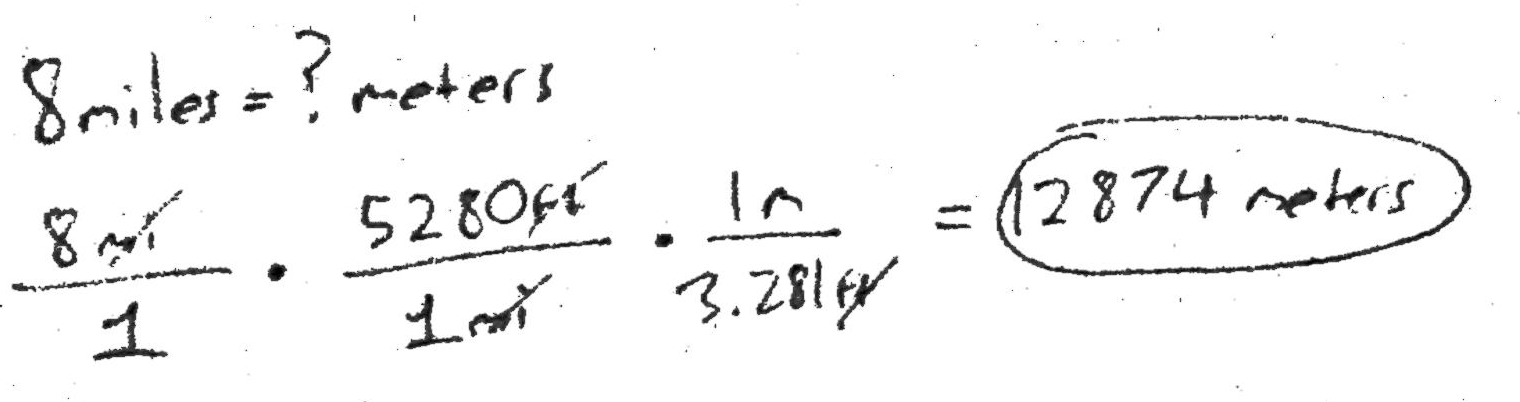
\includegraphics[width=0.8\textwidth]{U1_P1_A} % Example of adding a figure
\end{figure} \\

\newpage
\noindent\textbf{B) How long does it take Hancock to travel 8 miles if he maintains a speed of 30 m/s?} \\


\begin{figure}[H]
    \centering
    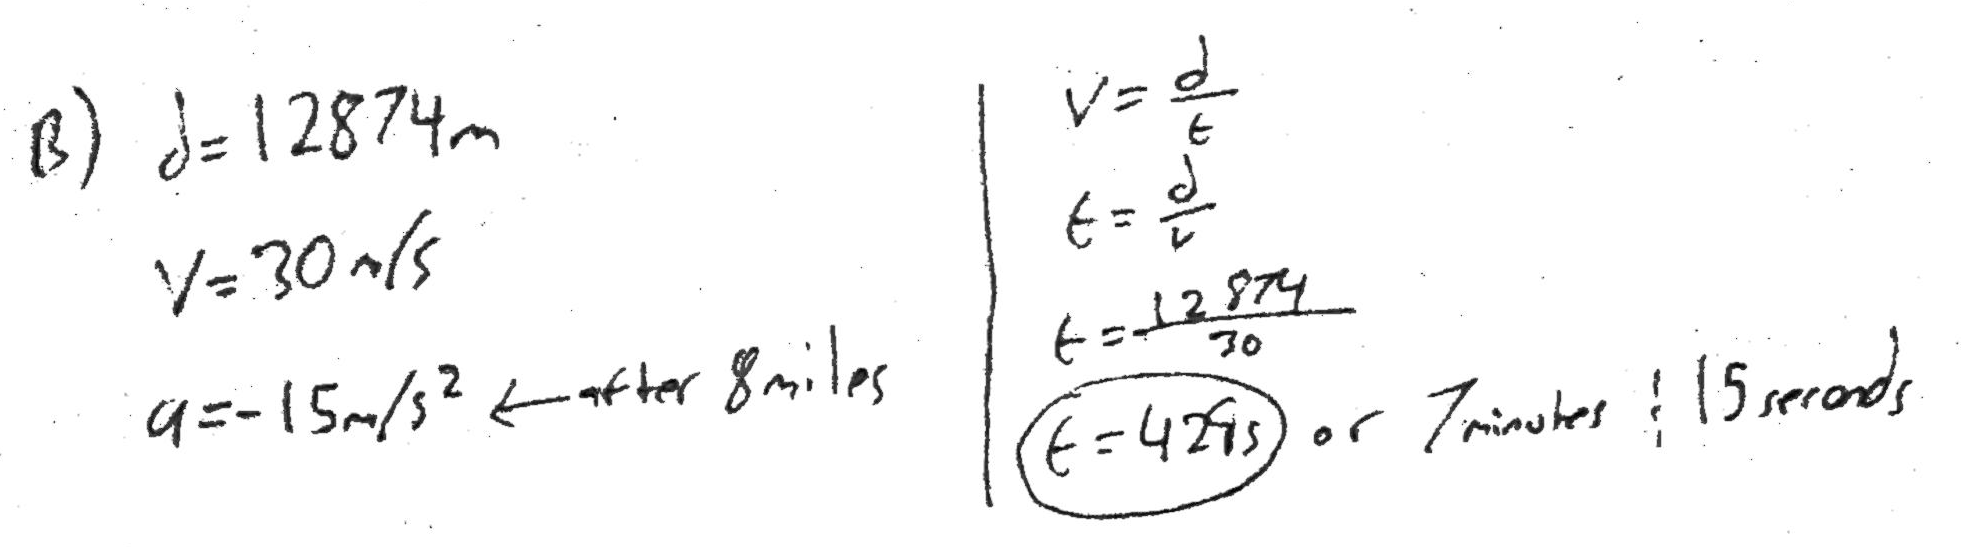
\includegraphics[width=0.8\textwidth]{U1_P1_B} % Example of adding a figure
\end{figure}


\noindent\textbf{C) Once he reaches the vehicle, how long does it take for Hancock to come to a complete stop with a deceleration of -15 m/s$^2$?} \\


\begin{figure}[H]
    \centering
    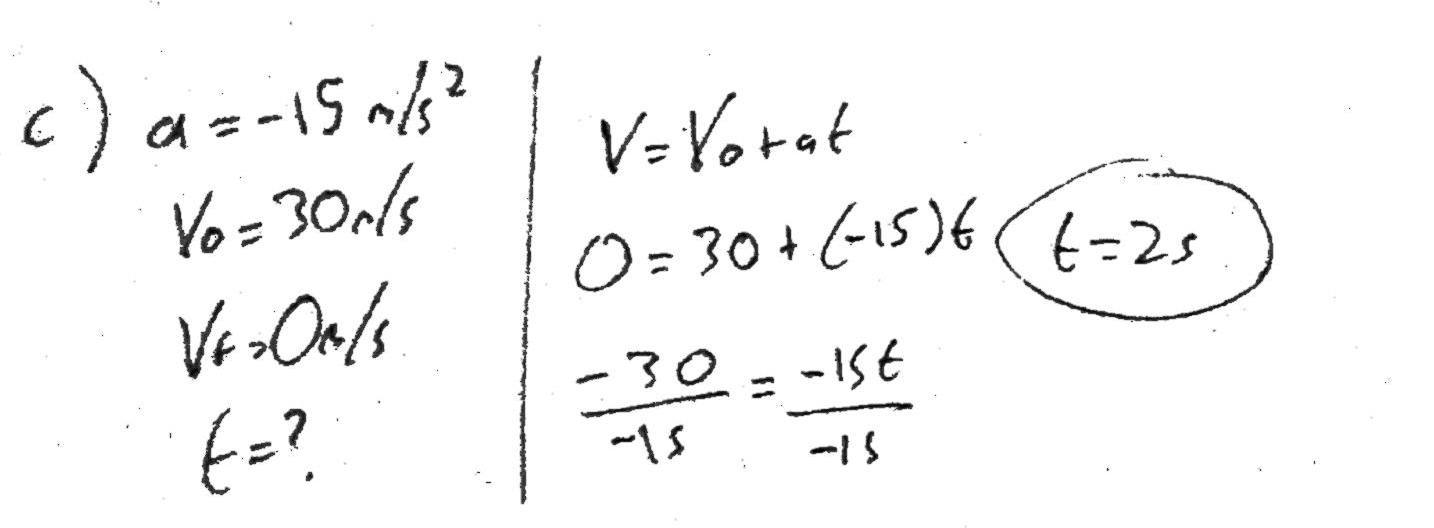
\includegraphics[width=0.8\textwidth]{U1_P1_C} % Example of adding a figure
\end{figure}

%-----------------PROBLEM 2--------------------------%

\newpage
\subsection{Problem 2}

Assume Hancock throws the car straight up into the air from the ground to scare the crooks at an initial velocity of 20 m/s. He catches the car a short time later. \\

\noindent\textbf{A) Calculate the car's acceleration immediately after Hancock releases it.} \\


\begin{figure}[H]
    \centering
    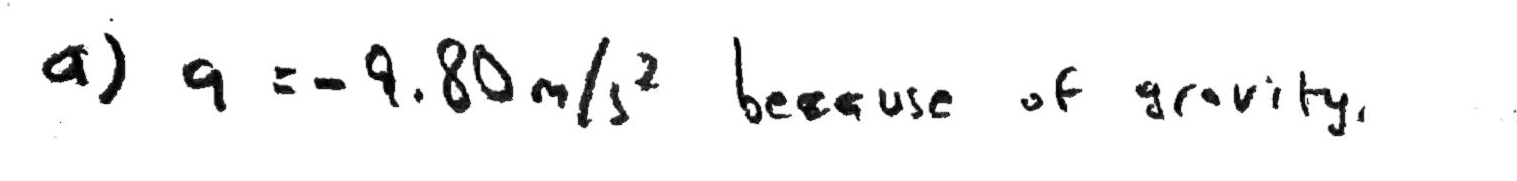
\includegraphics[width=0.8\textwidth]{U1_P2_A} % Example of adding a figure
\end{figure}


\noindent\textbf{B) Calculate the displacement of the car.} \\


\begin{figure}[H]
    \centering
    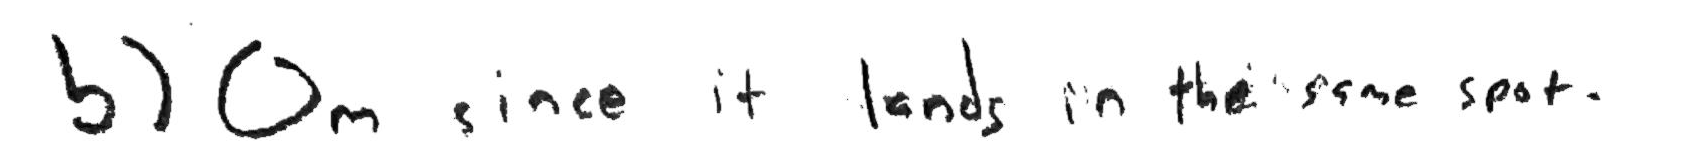
\includegraphics[width=0.8\textwidth]{U1_P2_B} % Example of adding a figure
\end{figure}

\noindent\textbf{C) Calculate the maximum height the car reaches above the ground.}\\ 


\begin{figure}[H]
    \centering
    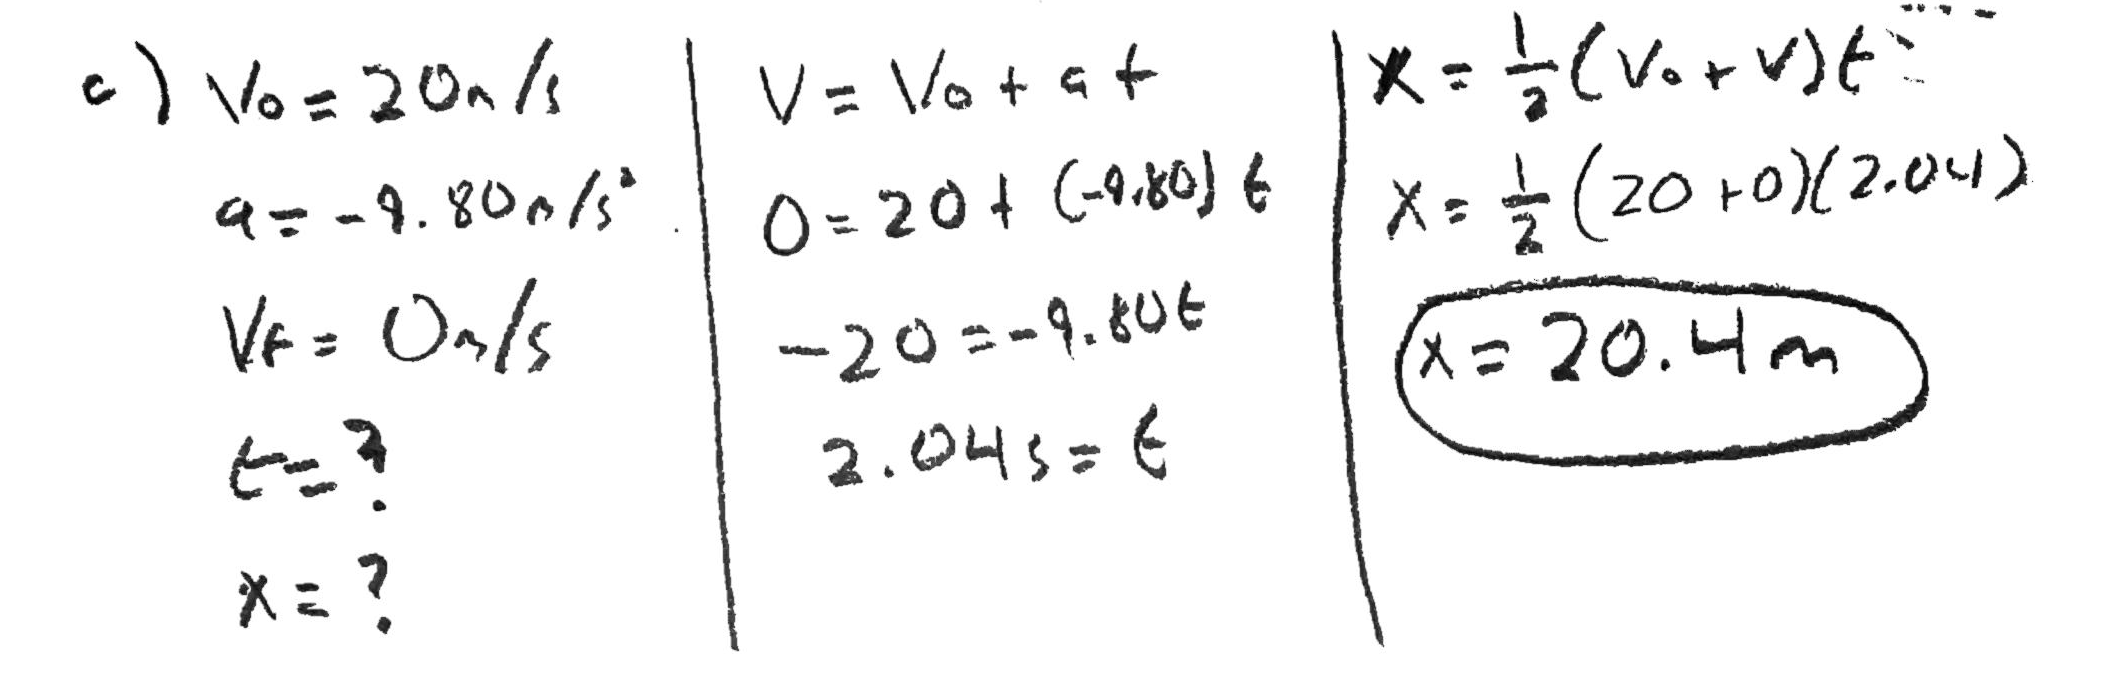
\includegraphics[width=0.8\textwidth]{U1_P2_C} % Example of adding a figure
\end{figure}

%\vspace{-0.5cm}

\noindent\textbf{D) How long does it take the car to reach its maximum height? What's the total time in the air?} \\

\vspace{-0.2cm}


\begin{figure}[H]
    \centering
    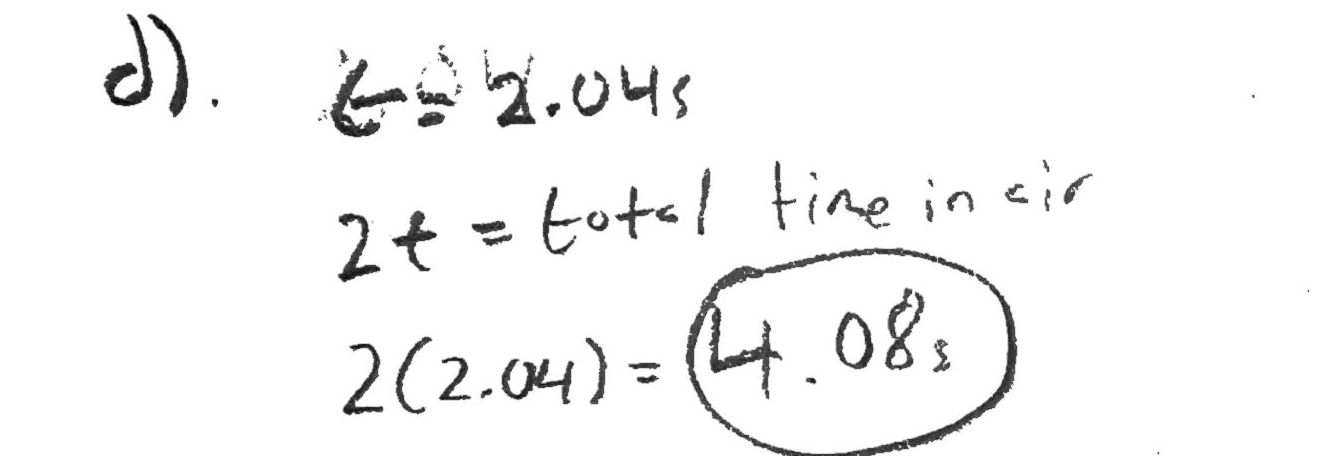
\includegraphics[width=0.8\textwidth]{U1_P2_D} % Example of adding a figure
\end{figure}

\newpage

%==============UNIT 2==================%

\section{Unit 2}

\vspace{-0.5cm}
\singlespacing

\subsection{Scene Analysis}

\textbf{Duration}: 26:00 - 28:00

\vspace{0.3cm}
\noindent\textbf{Summary:} \par
After being taunted by a 10 year old, Hancock loses his patience and throws the kid into the air. While in the air, Hancock finishes a conversation and walks a short distance, positioning himself to catch the child just before he hits the ground.
\par


\vspace{0.3cm}
\noindent\textbf{Concepts Demonstrated} \par
This scene is an excellent example of kinematics in two dimensions. Hancock accounts for the horizontal distance that the kid travels in the air to catch him at just the right moment.  


\subsection{Problem 1}
Assume Hancock throws the child vertically upward with an initial velocity of 58 m/s at an angle of 87$^\circ$. Neglect air resistance. \\


\noindent\textbf{A) Calculate the initial vertical and horizontal components of the child's velocity.} \\


\begin{figure}[H]
    \centering
    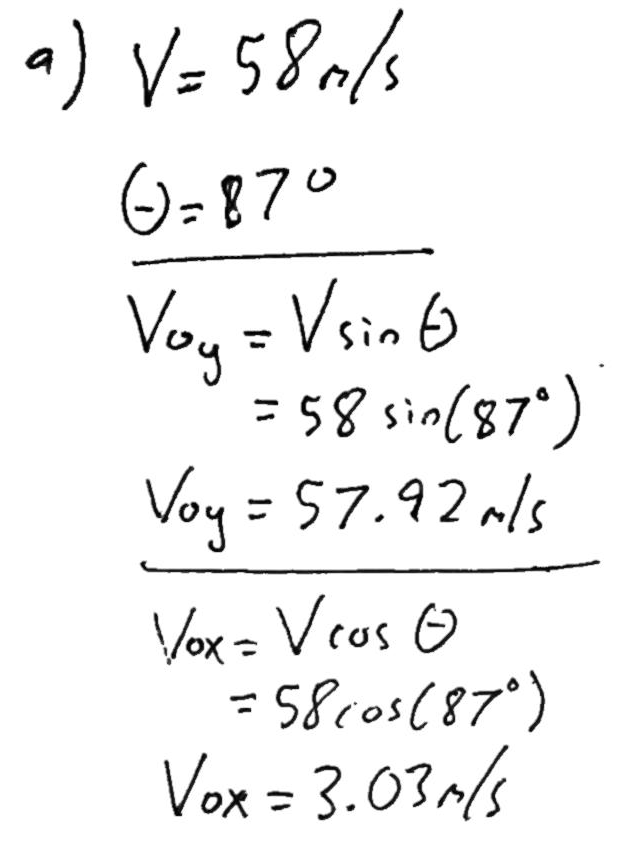
\includegraphics[width=0.3\textwidth]{U2_P1_A} % Example of adding a figure
\end{figure}

\newpage

\noindent\textbf{B) Calculate the maximum height the child reaches. \emph{Could he see his house from up there?}} \\

\vspace{-0.5cm}

\begin{figure}[H]
    \centering
    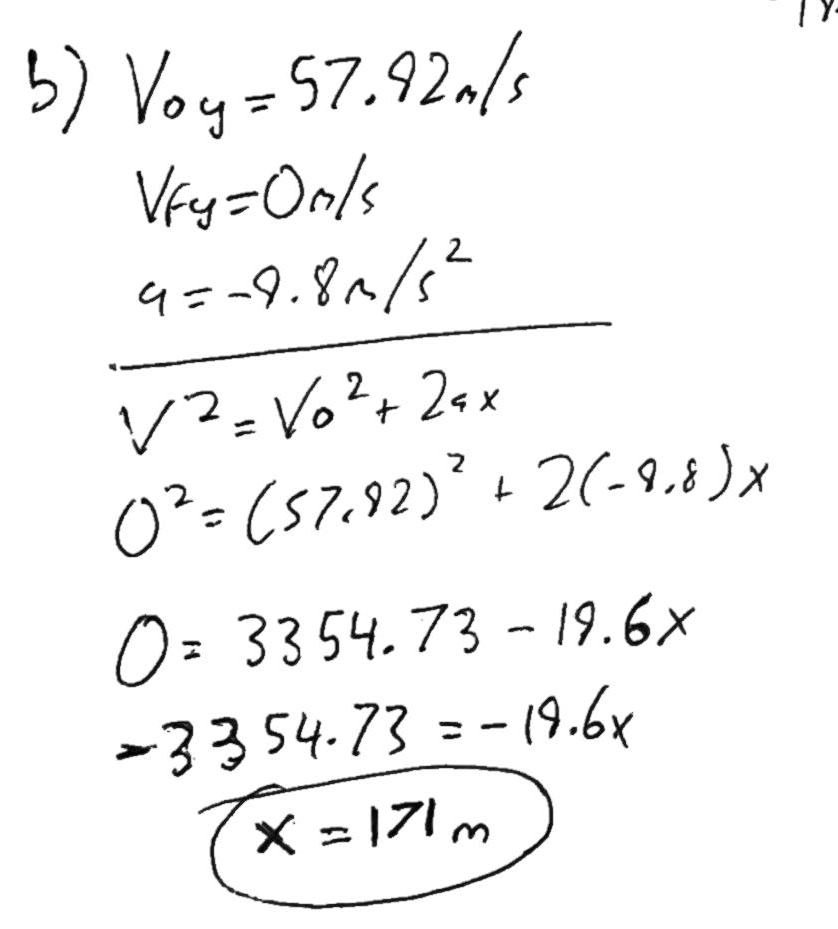
\includegraphics[width=0.4\textwidth]{U2_P1_B} % Example of adding a figure
\end{figure}

\noindent\textbf{C) How long does it take the child to reach maximum height? And to come back down? \emph{Is that enough time to think about the mistake he made?}} \\

\vspace{-0.5cm}

\begin{figure}[H]
    \centering
    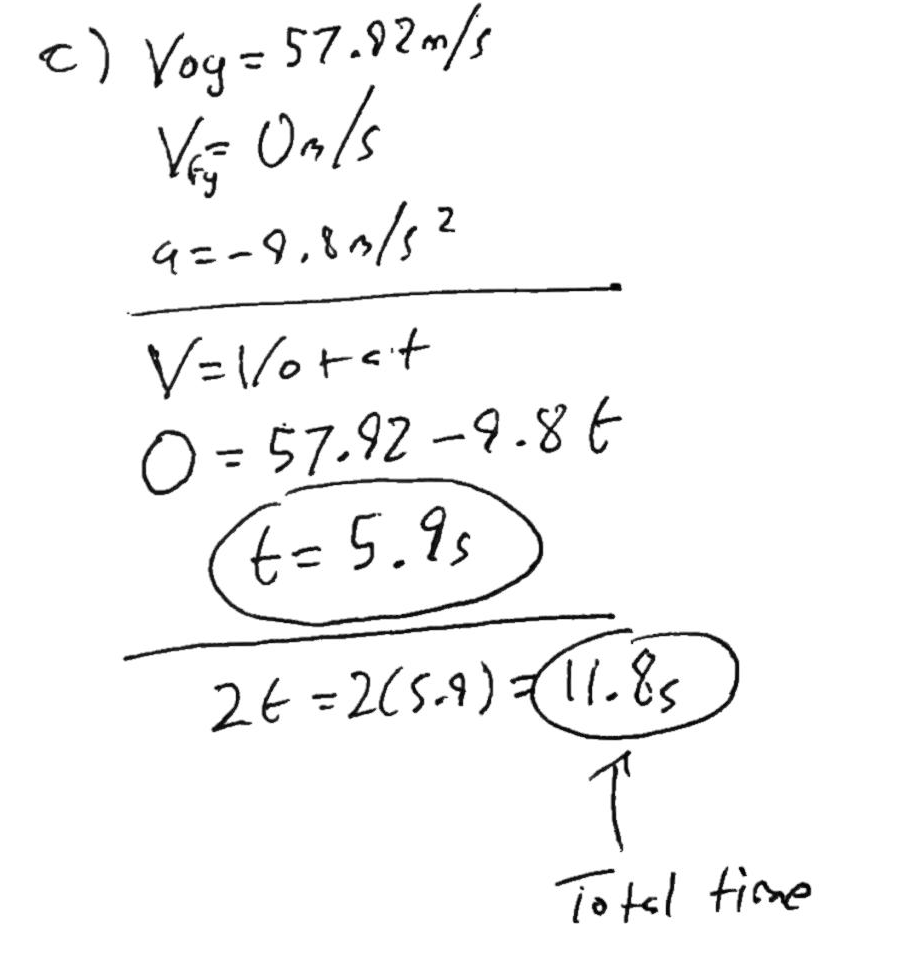
\includegraphics[width=0.4\textwidth]{U2_P1_C} % Example of adding a figure
\end{figure}

\noindent\textbf{D) How far does Hancock have to walk to catch the kid?} \\

\vspace{-0.5cm}

\begin{figure}[H]
    \centering
    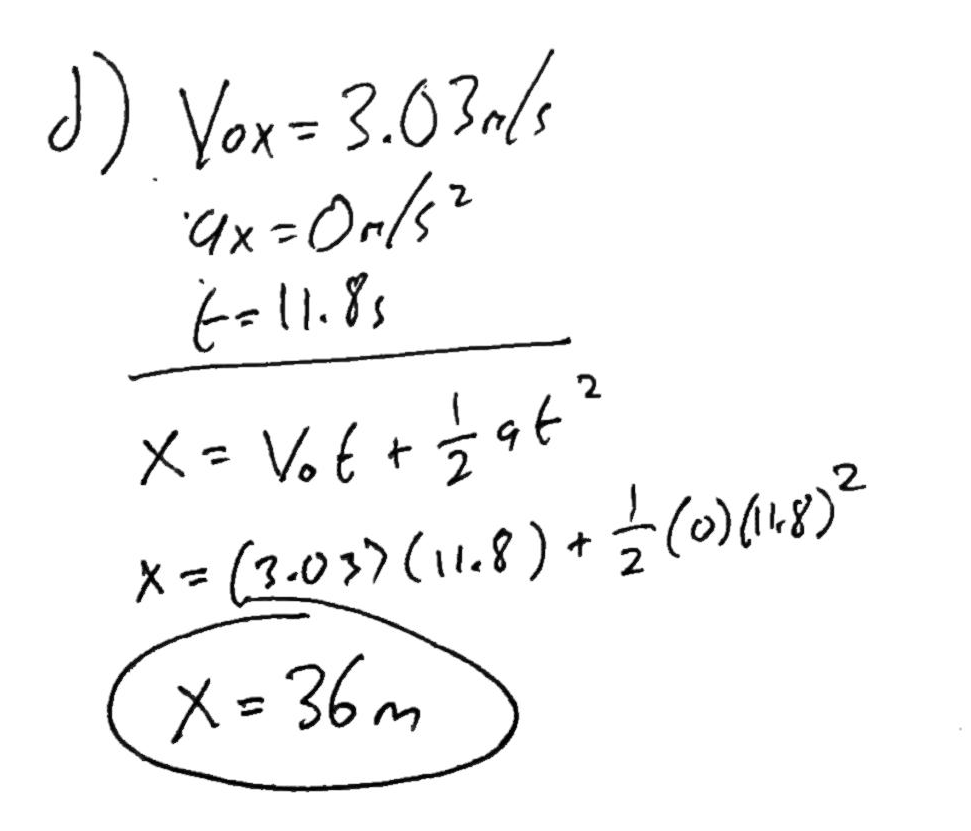
\includegraphics[width=0.4\textwidth]{U2_P1_D} % Example of adding a figure
\end{figure}

\subsection{Problem 2}

Hancock messes up his calculations and the kid ends up falling a distance 10 meters away from him. Using his super speed, Hancock runs and catches the kid before he hits the ground. Assume Hancock has a mass of 85 kg, moves with an initial velocity of 5 m/s, and slides to slow down and catch the child with a net acceleration of 3 m/s$^2$ that brings him to rest over a distance of 3 meters. 
\\

\noindent\textbf{A) Calculate the magnitude of the friction force acting on Hancock during the slide. What's the coefficient of friction between Hancock and the ground? How long does it take for Hancock to come to rest?} \\


\begin{figure}[H]
    \centering
    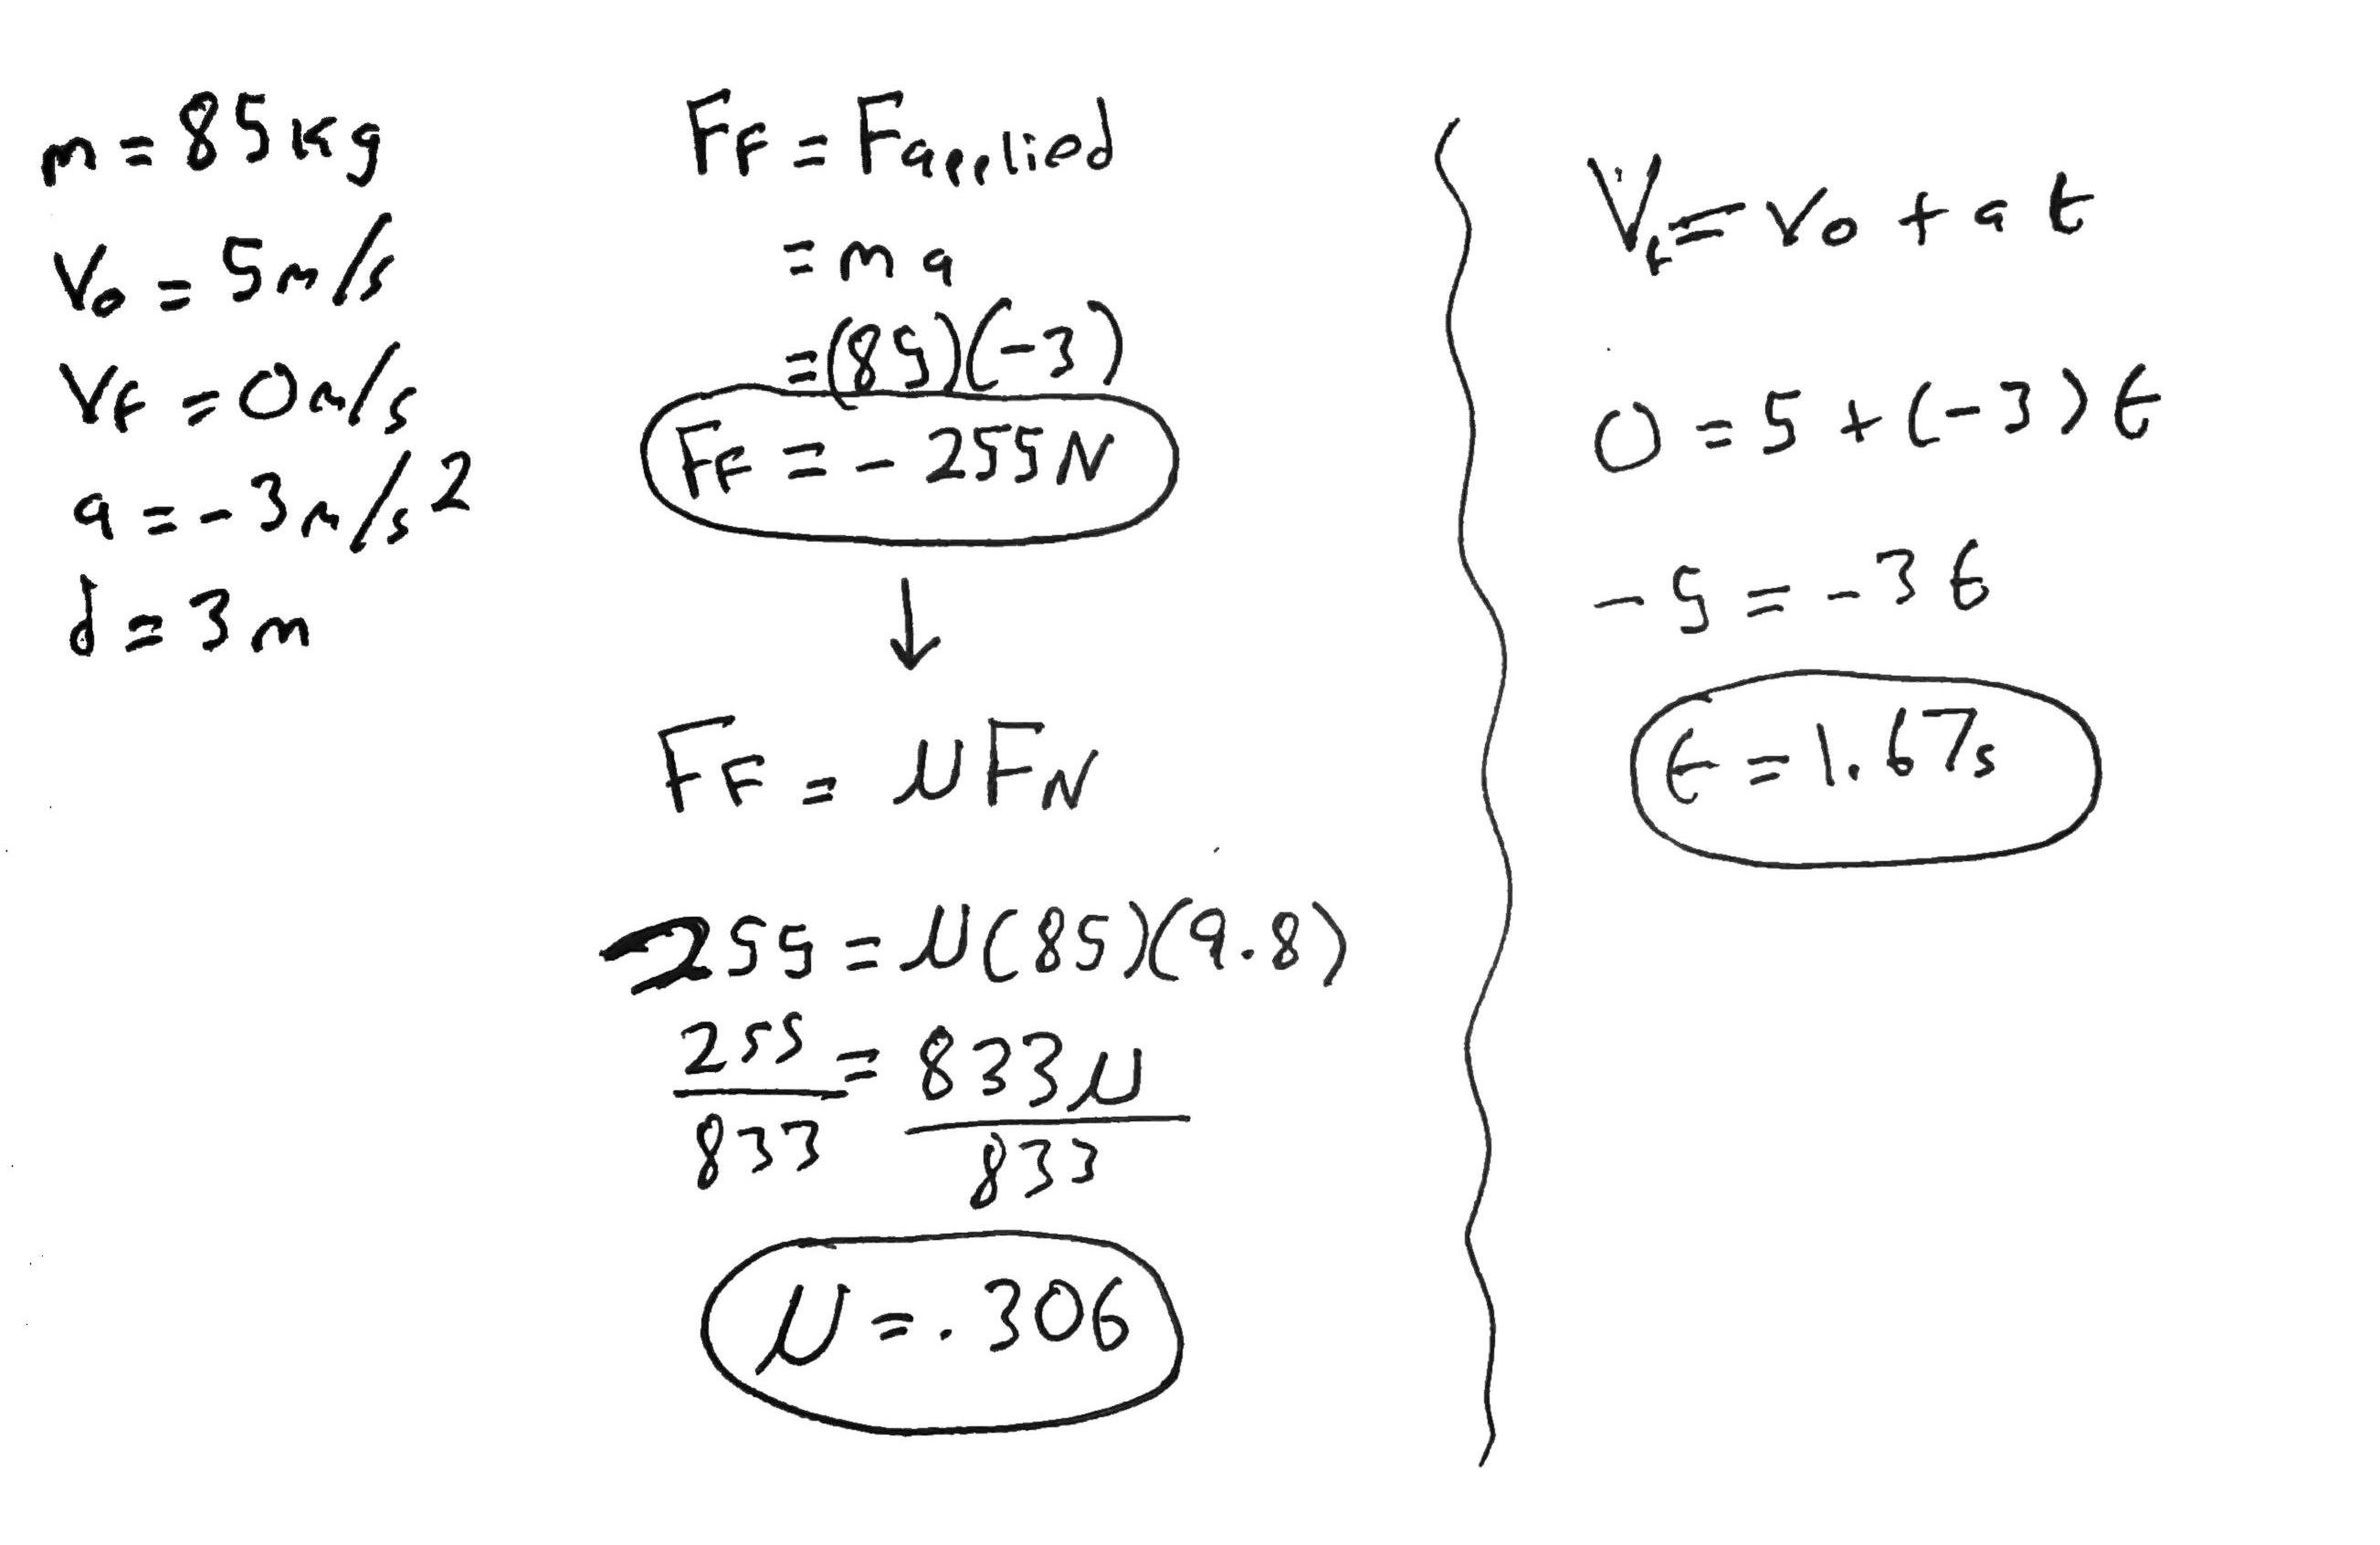
\includegraphics[width=0.6\textwidth]{U2_P2_A.jpg} % Example of adding a figure
\end{figure}


\noindent\textbf{B)Which of the following FBDs correctly represents Hancock during the sliding portion of his motion? } \\


\begin{figure}[H]
    \centering
    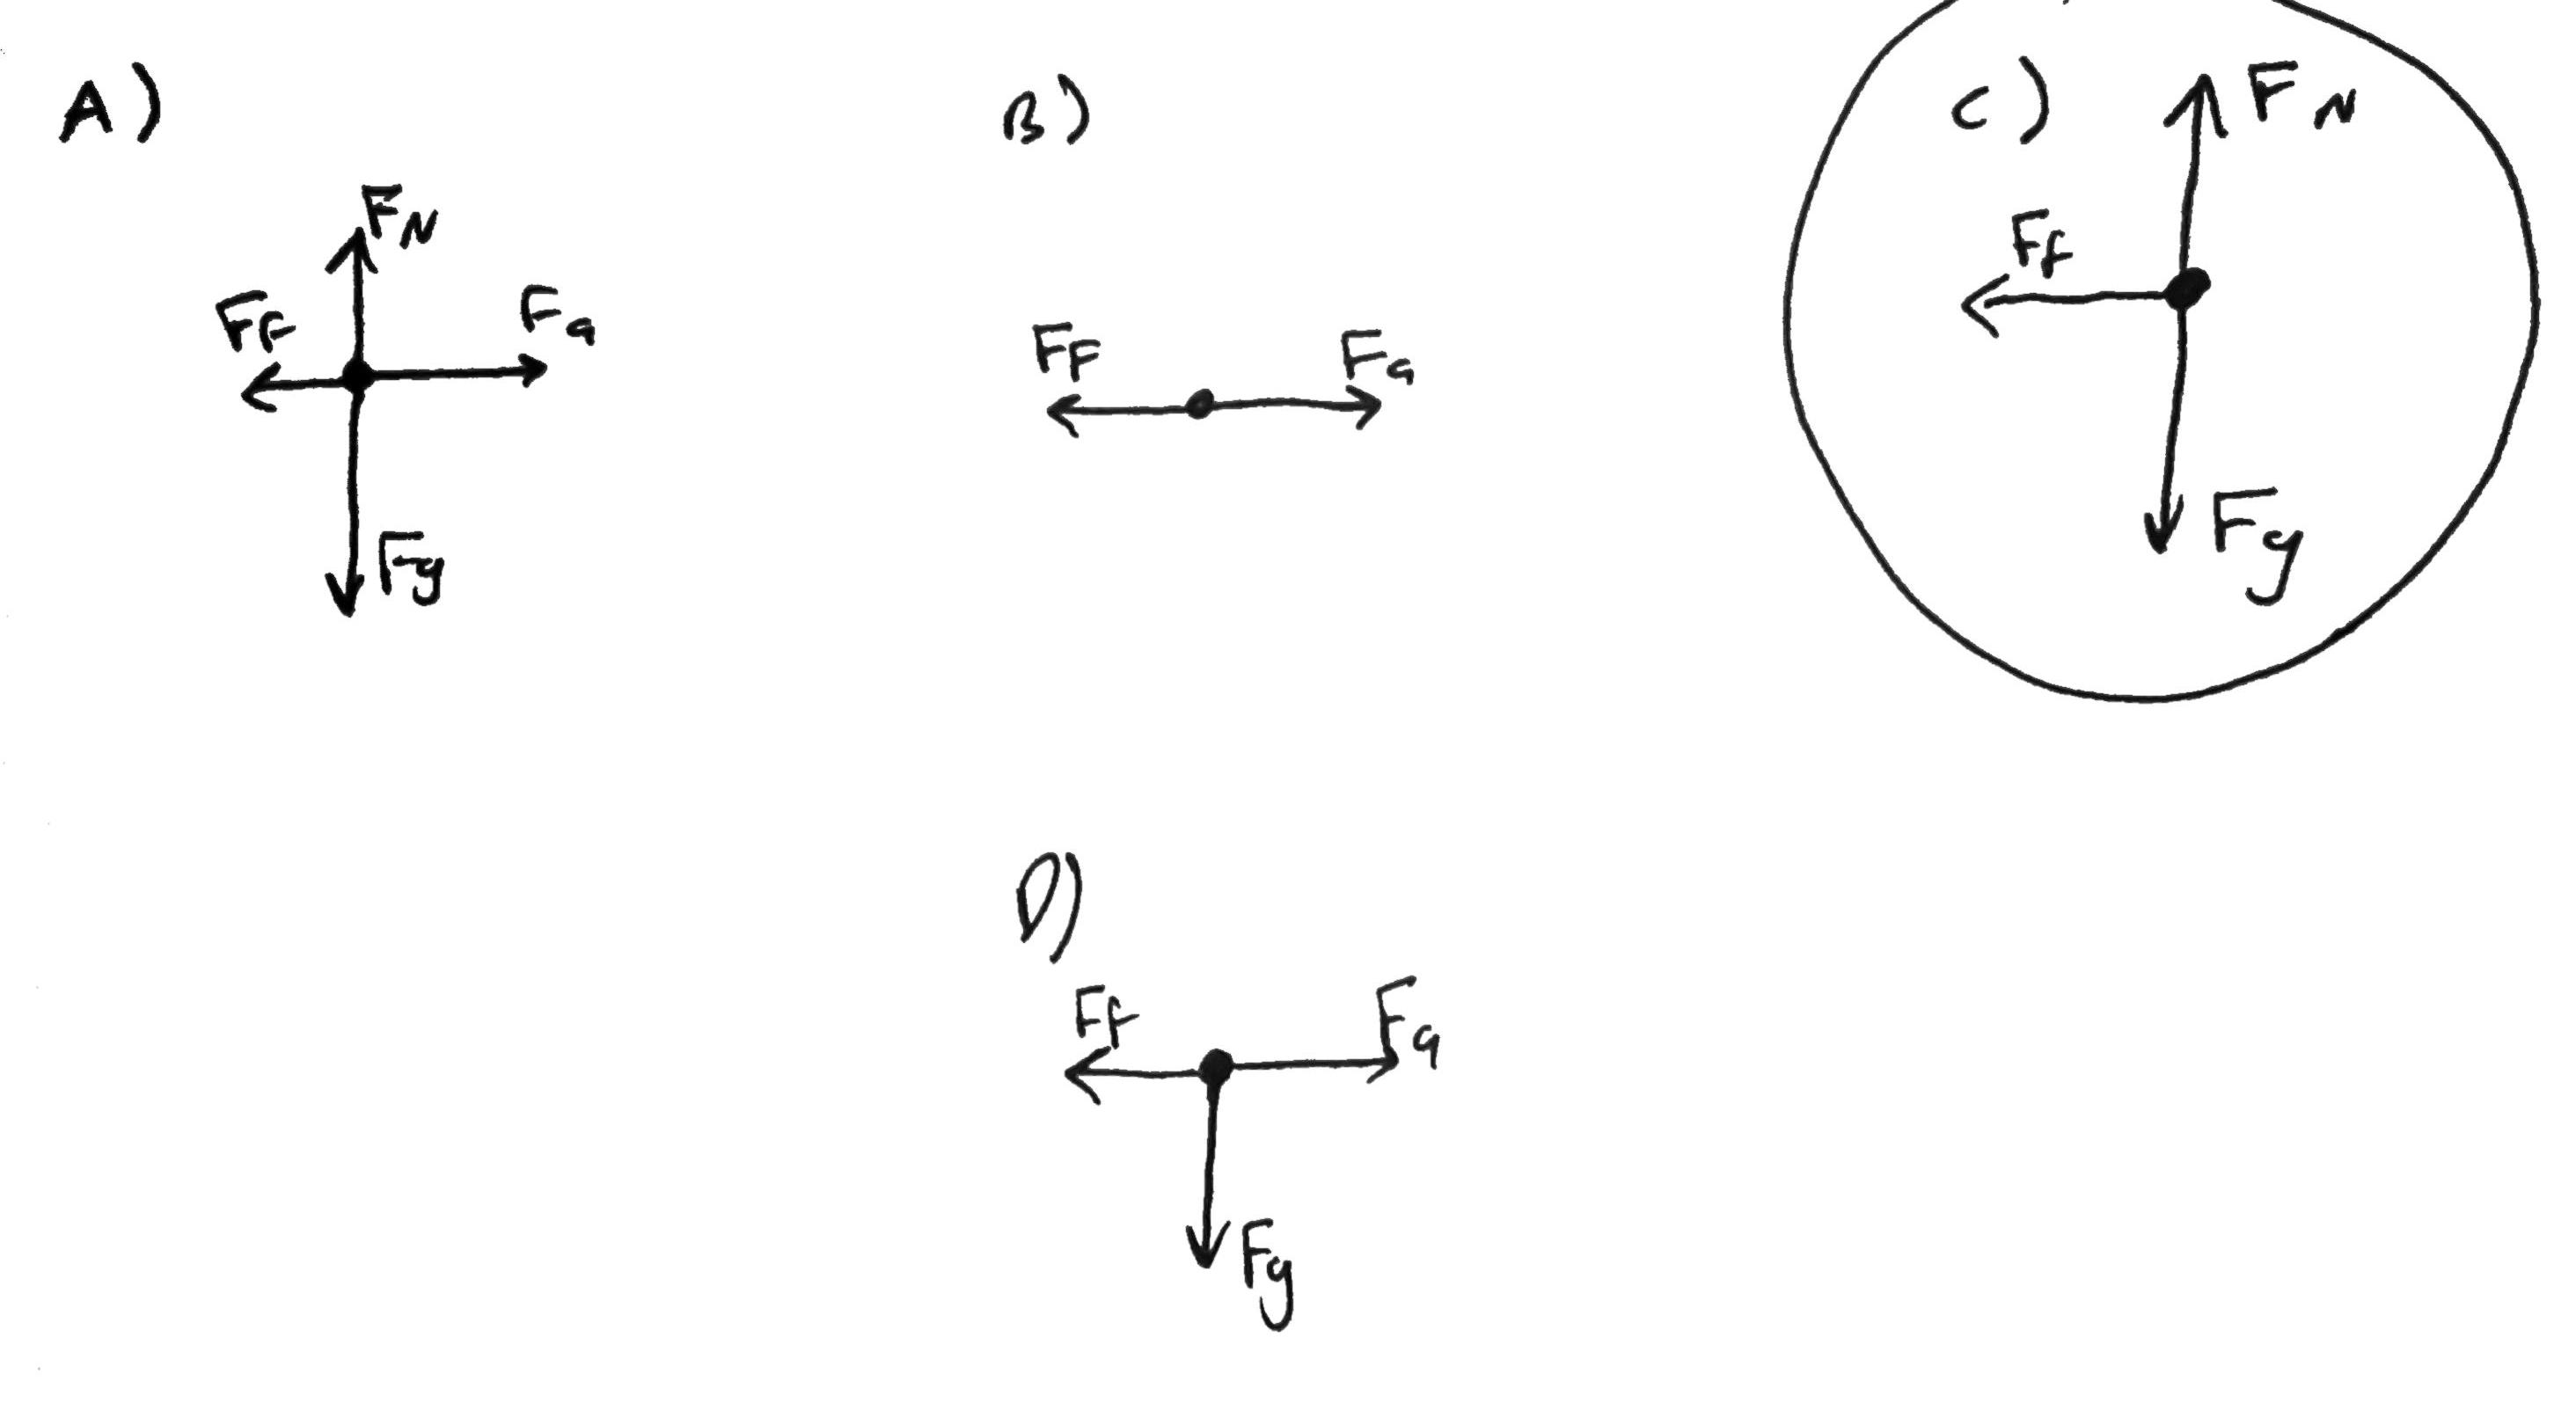
\includegraphics[width=0.8\textwidth]{U2_P2_B.jpg} % Example of adding a figure
\end{figure}

\newpage


%=====================UNIT 3===================%
\section{Unit 3}

\vspace{-0.5cm}
\singlespacing

\subsection{Scene Analysis}

\textbf{Duration}: 17:54 - 24:00

\vspace{0.3cm}
\noindent\textbf{Summary:} \par
After preventing a train from hitting the car of public relations manager, Ray, Hancock carries the car back to Ray's house. When he arrives, he drags the car up a slight incline into the garage. \\
\par


\vspace{0.3cm}
\noindent\textbf{Concepts Demonstrated} \par
This scene demonstrates work done by a force, kinetic energy and gravitational potential energy as Hancock drags the car up to Ray's garage.  

\subsection{Problem 1}
Assume Hancock drags Ray's 1500 kg car up a 5$^\circ$ incline over a distance of 50 m to the garage. The frictional force opposing the motion is 3000 N, and Hancock maintains a constant speed of 4 m/s as he moves the car up the incline. \\


\noindent\textbf{A) Calculate the work done by Hancock to overcome the frictional force as he drags the car up the incline.} \\


\begin{figure}[H]
    \centering
    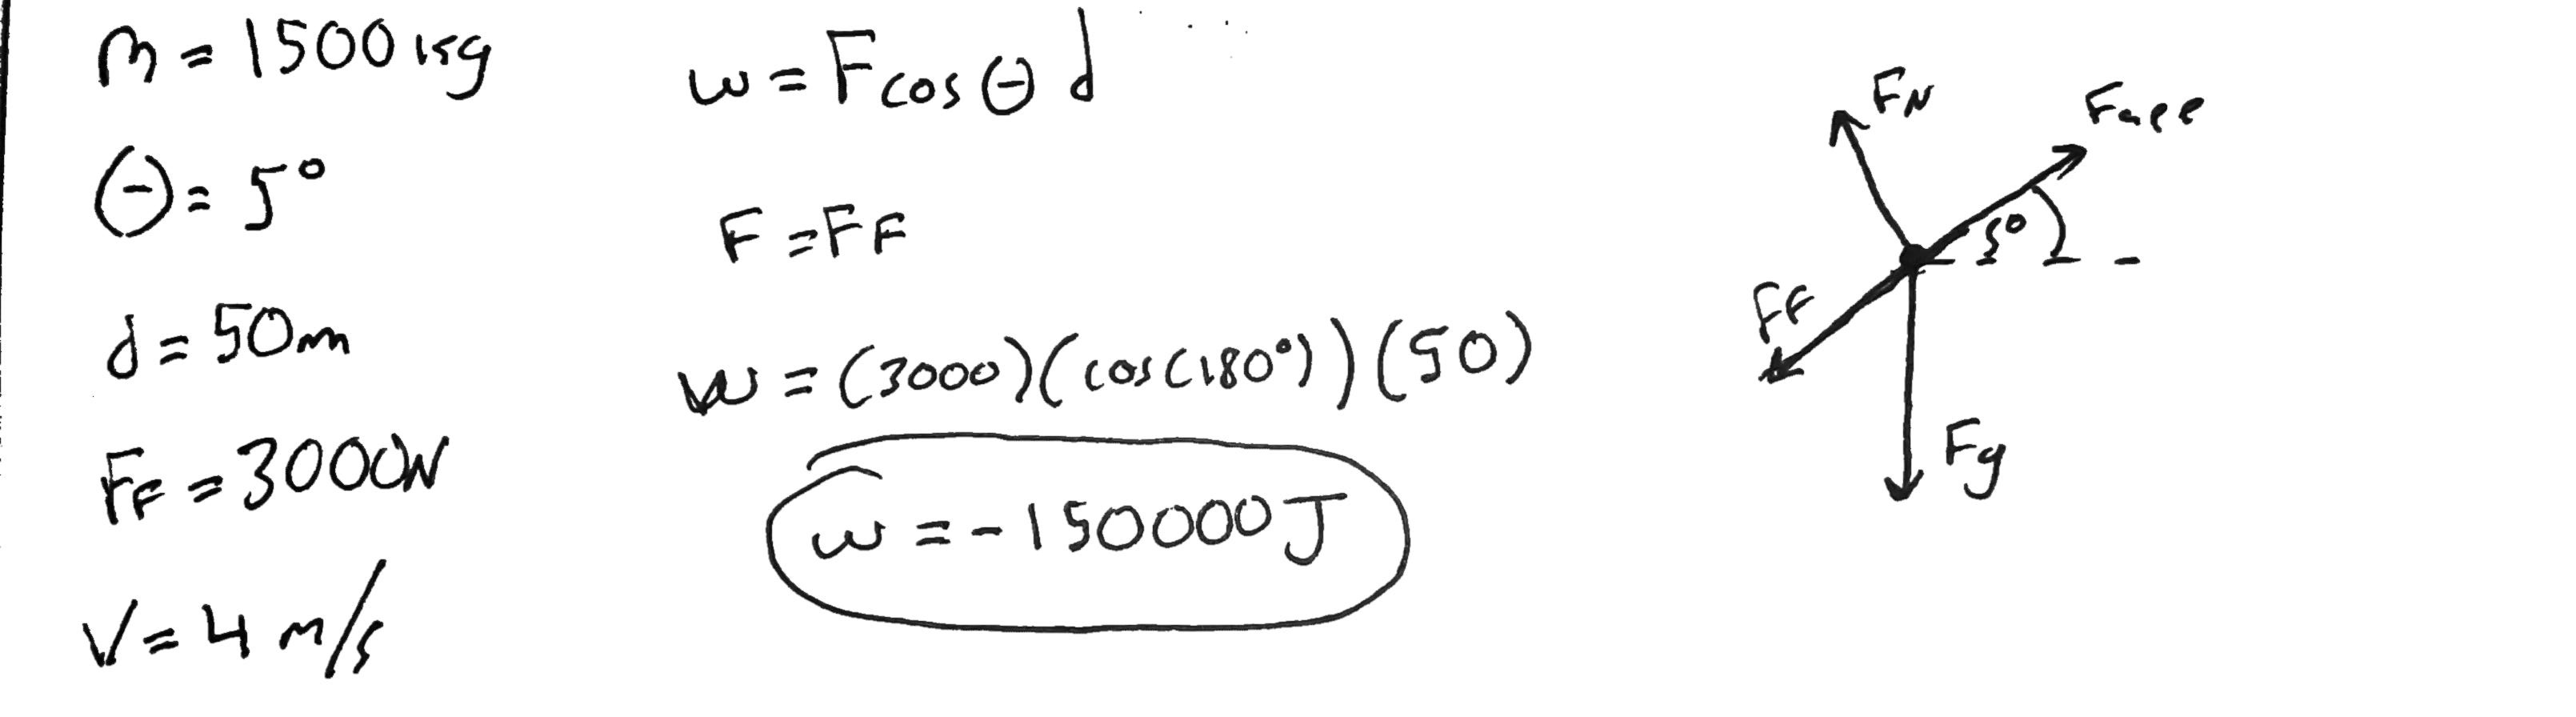
\includegraphics[width=0.9\textwidth]{U3_P1_A.jpg} % Example of adding a figure
\end{figure} 

\newpage

\noindent\textbf{B) Calculate the change in gravitational potential energy of the car as it is raised to the height of the incline.} \\


\begin{figure}[H]
    \centering
    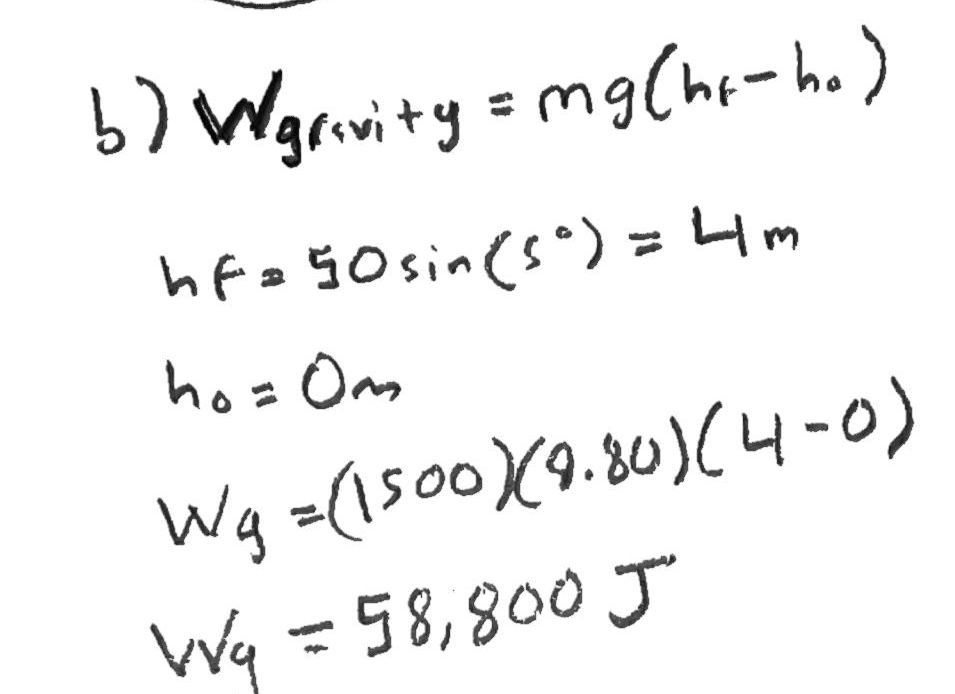
\includegraphics[width=0.5\textwidth]{U3_P1_B} % Example of adding a figure
\end{figure}

\noindent\textbf{C) Calculate the total work Hancock performs to move the car up the incline.} \\


\begin{figure}[H]
    \centering
    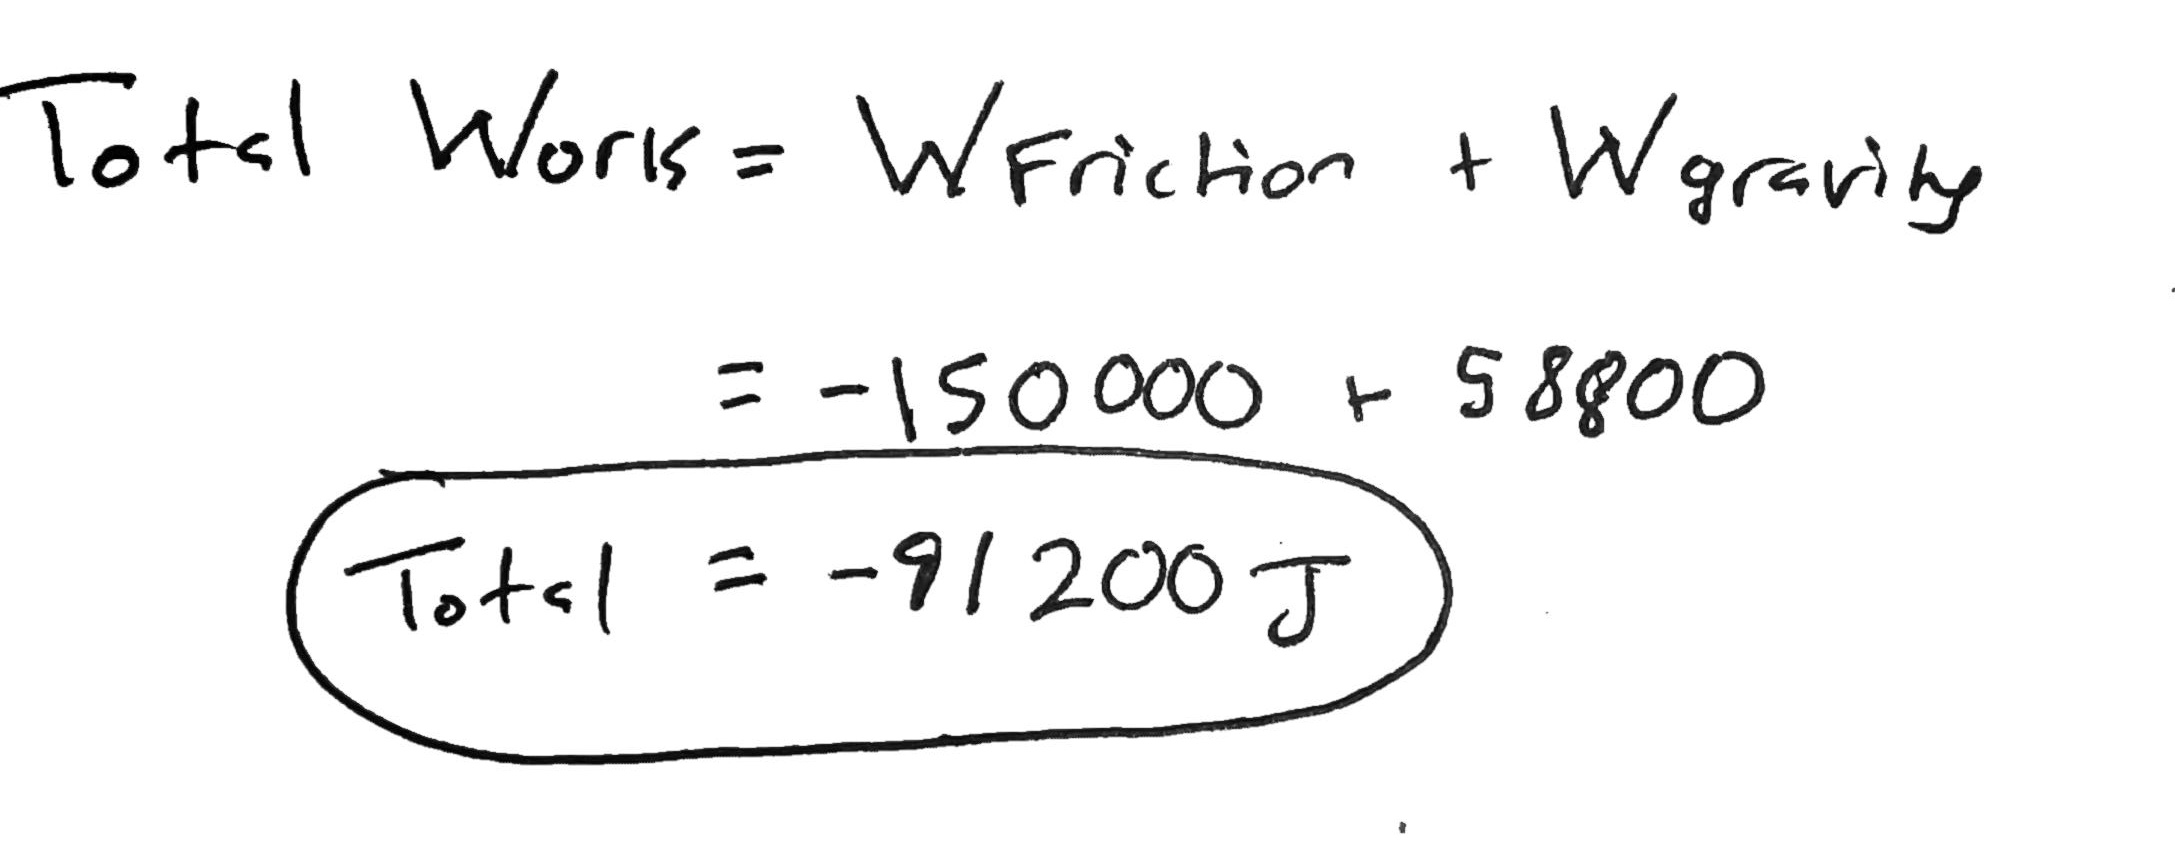
\includegraphics[width=0.6\textwidth]{U3_P1_C.jpg} % Example of adding a figure
\end{figure}

\noindent\textbf{D) Draw an FBD diagram of the car as it's dragged up the incline.} \\


\begin{figure}[H]
    \centering
    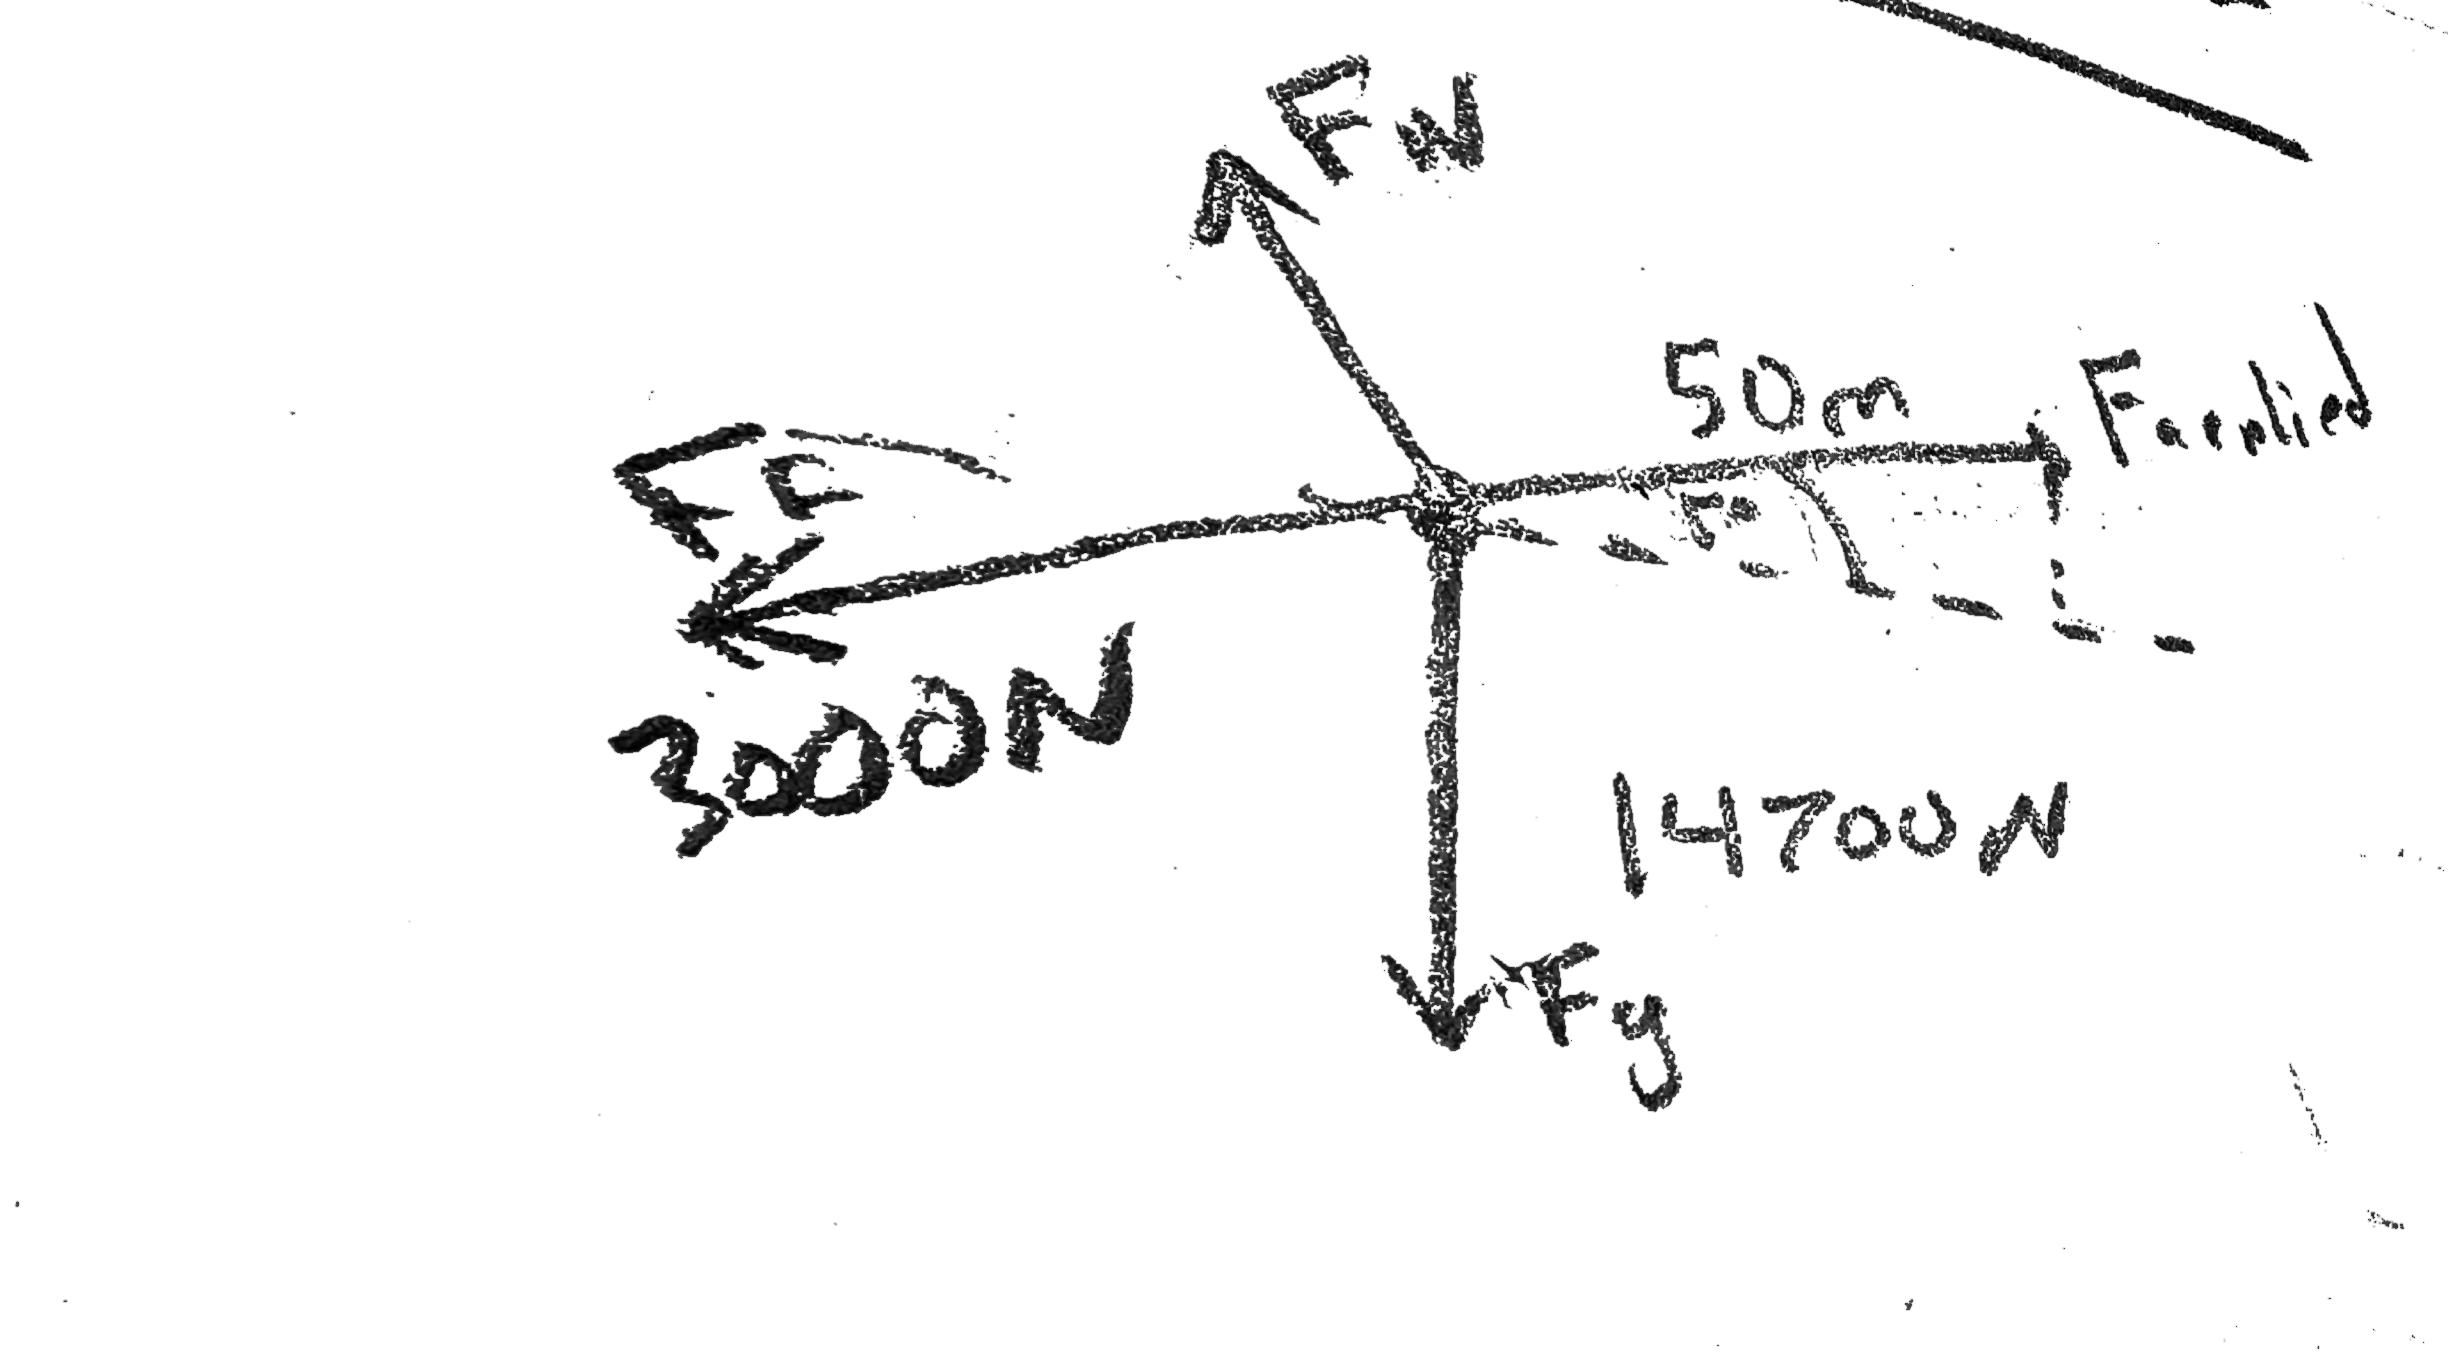
\includegraphics[width=0.5\textwidth]{U3_P1_F} % Example of adding a figure
\end{figure} 

\newpage 

\subsection{Problem 2}

To reorient the car so that it's placed into the garage with its hood facing the entrance, Hancock decides to quickly drag the car around in a circular path. The car has a mass of 1500 kg and, the radius of the circle Hancock makes is 3 meters. 


\noindent\textbf{A) Assume the car moves at a constant speed of 4 m/s while spinning: Calculate the centripetal force of the car} \\


\begin{figure}[H]
    \centering
    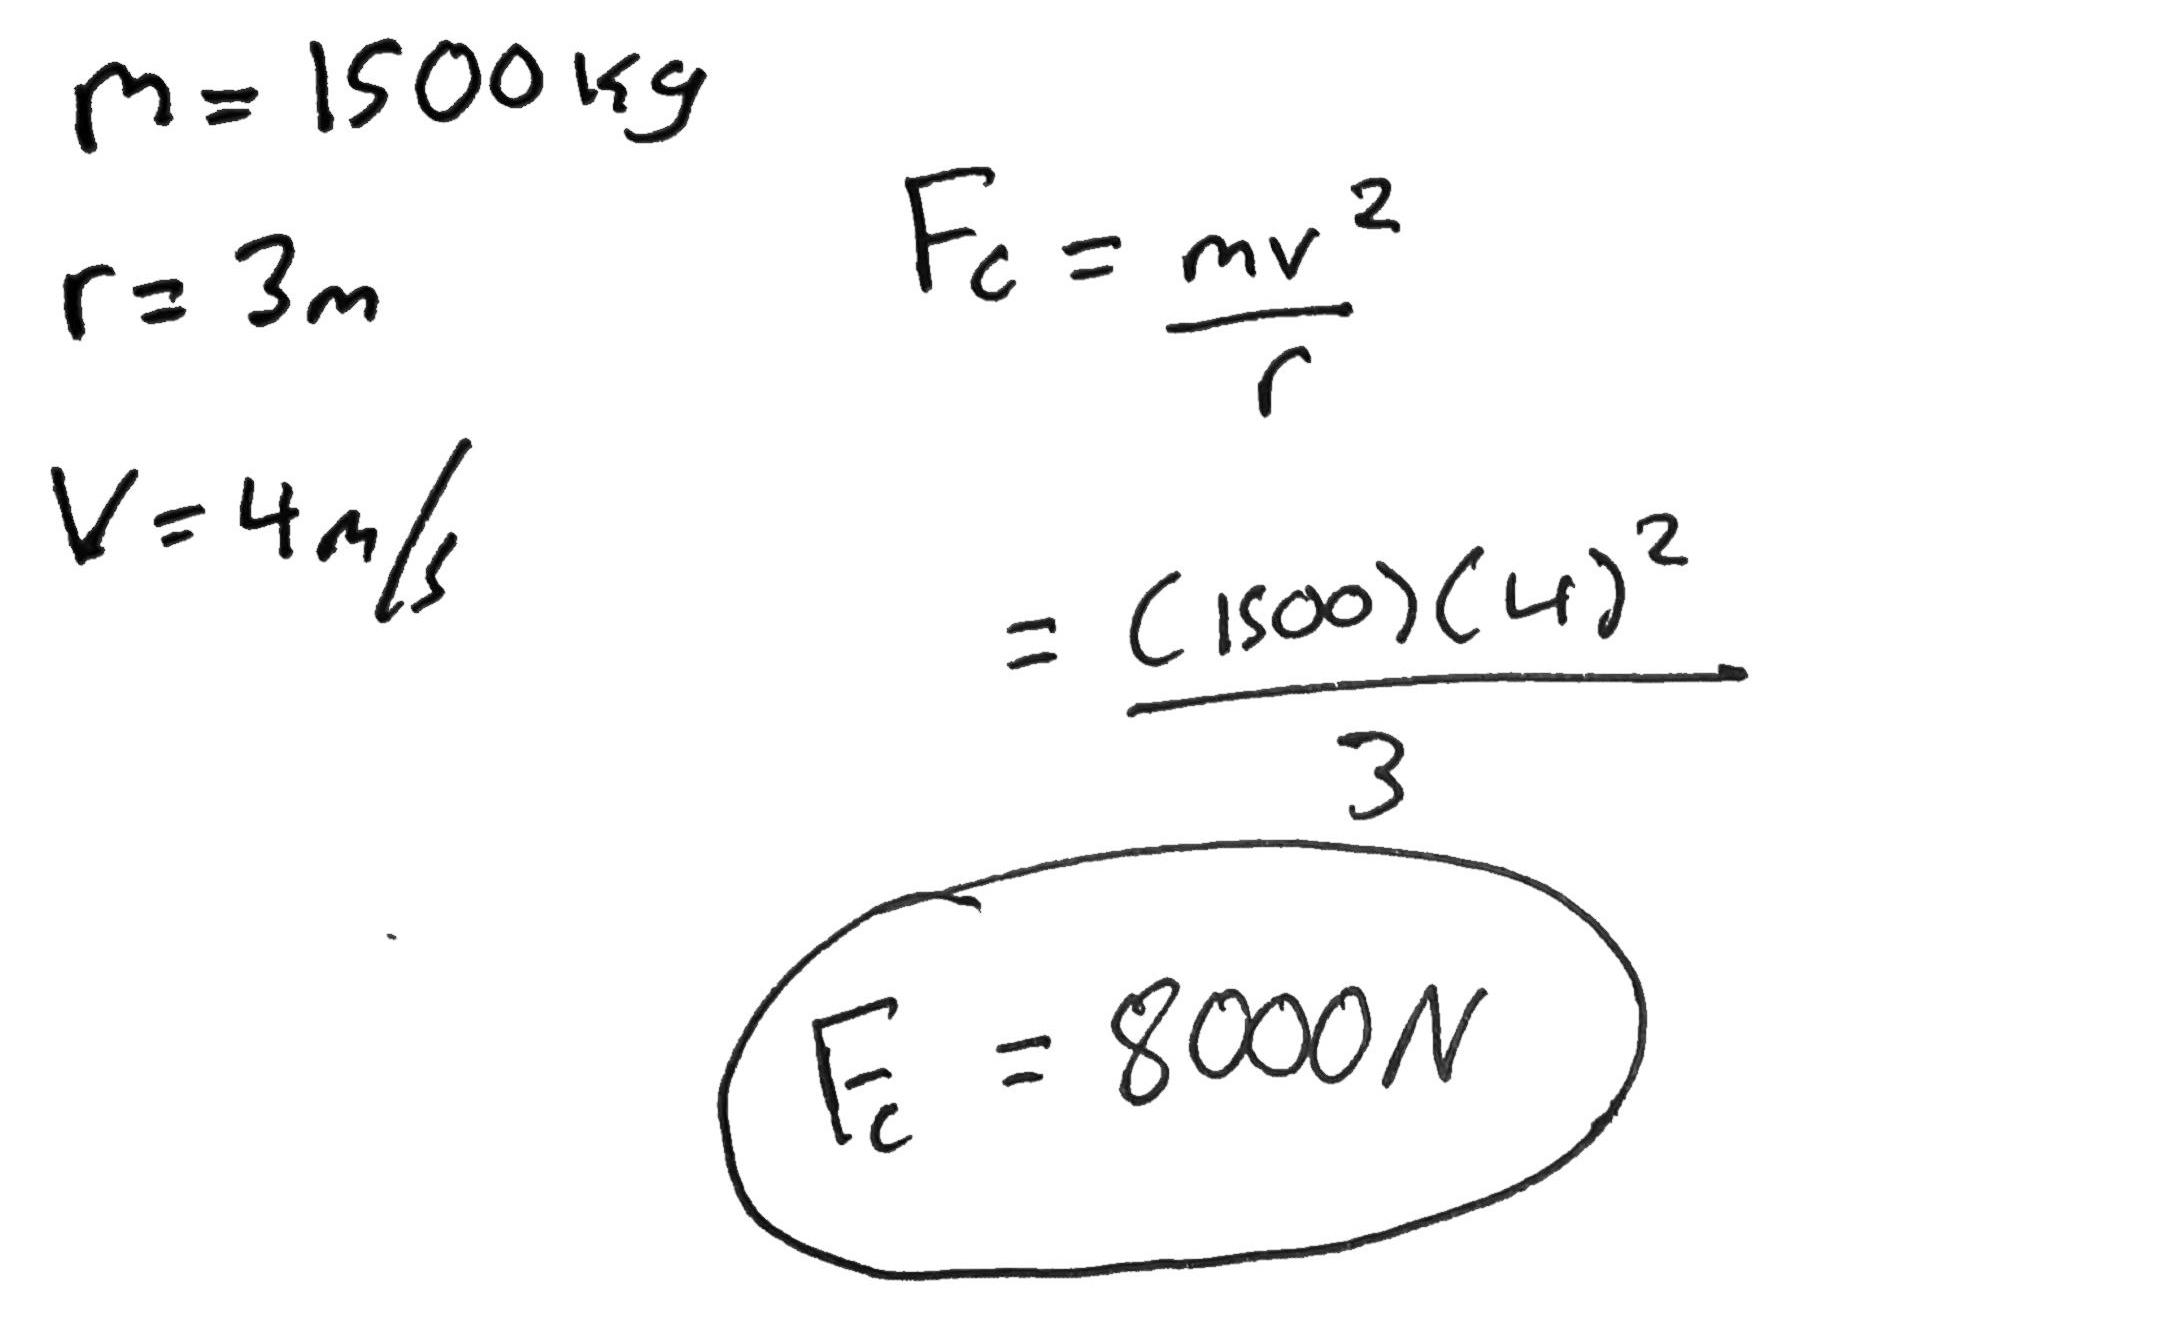
\includegraphics[width=0.6\textwidth]{U3_P2_A.jpg} % Example of adding a figure
\end{figure} 

\noindent\textbf{B) What force is providing the centripetal force? What is its magnitude?} \\

\begin{figure}[H]
    \centering
    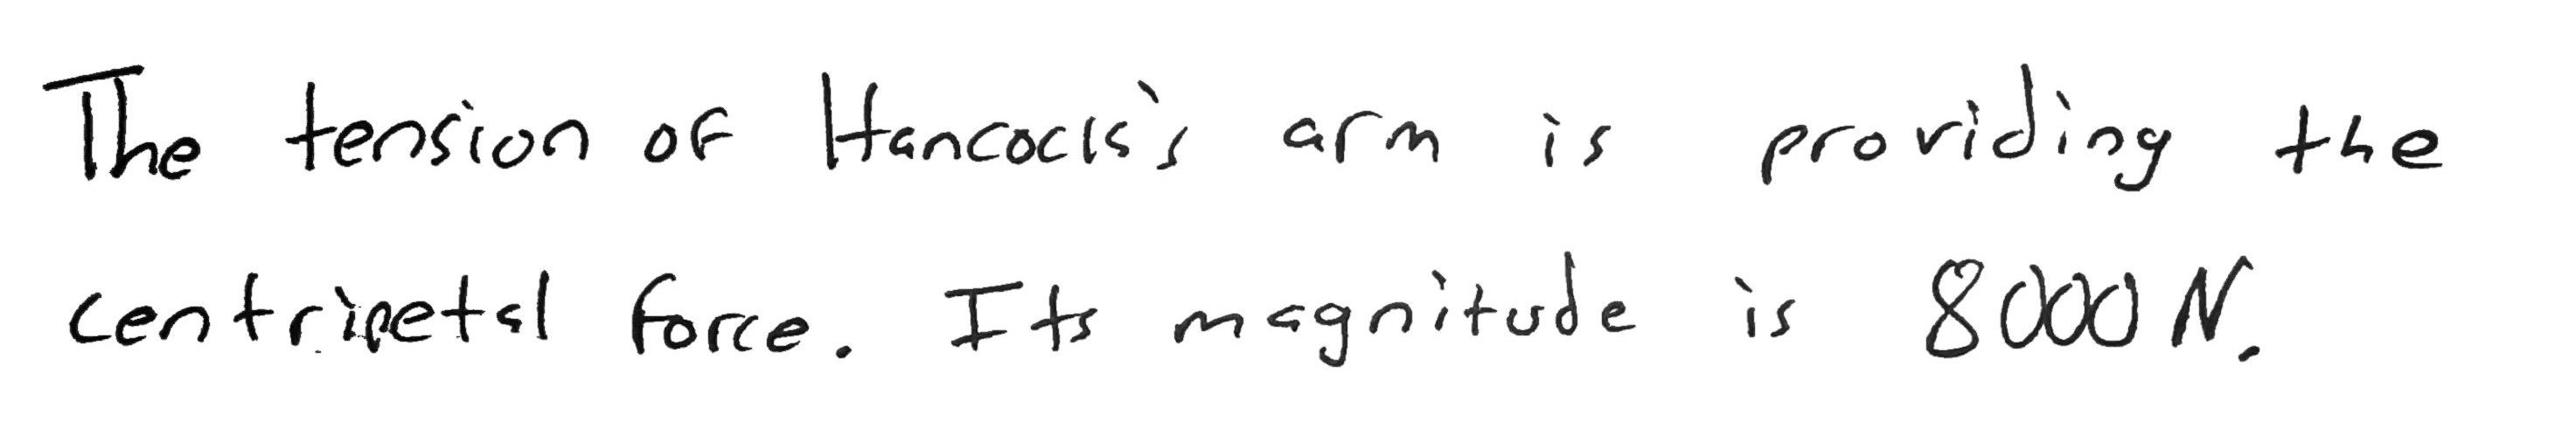
\includegraphics[width=1\textwidth]{U3_P2_B.jpg} % Example of adding a figure
\end{figure} 


\noindent\textbf{C) Draw an FBD diagram of car while it's spinning.} \\

\begin{figure}[H]
    \centering
    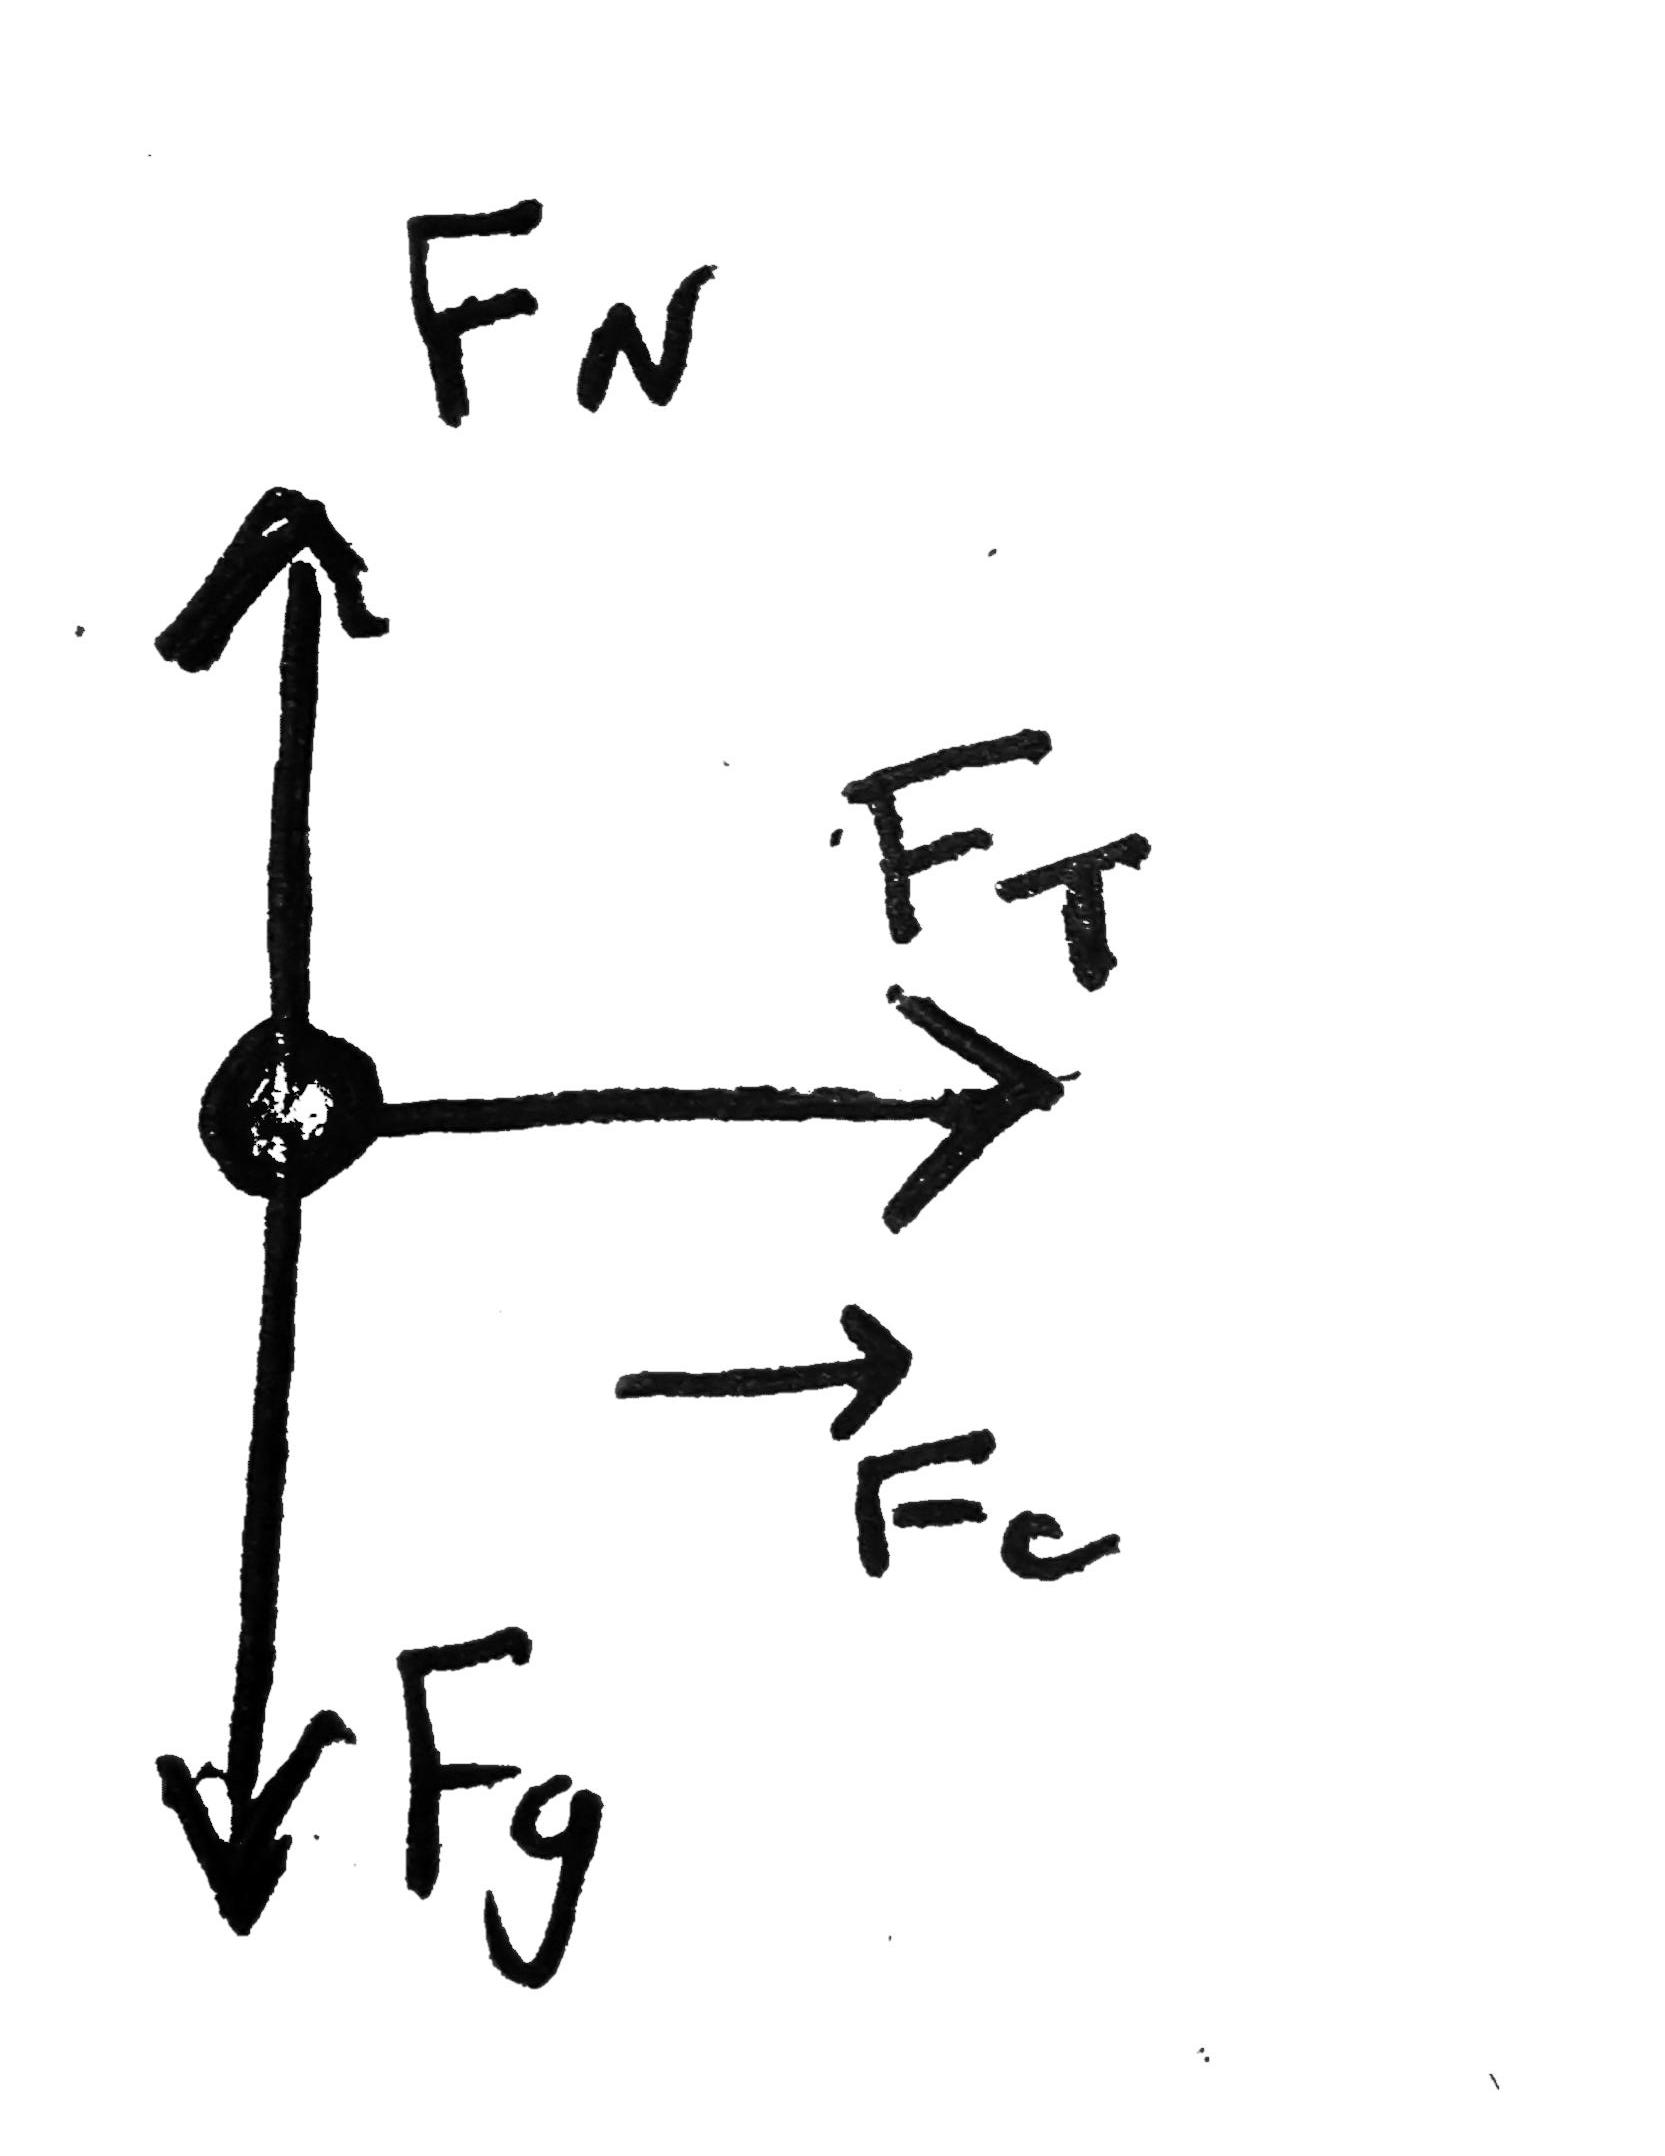
\includegraphics[width=0.3\textwidth]{U3_P2_C.jpg} % Example of adding a figure
\end{figure} 


\\




\newpage
%=====================UNIT 4===================%

\section{Unit 4}

\vspace{-0.5cm}
\singlespacing

\subsection{Scene Analysis}

\textbf{Duration}: 15:18 - 17:00

\vspace{0.3cm}
\noindent\textbf{Summary:} \par
Social media manager, Ray, after a bad day at work, later finds himself stuck in traffic, right in the path of an incoming train. Hancock shows up just in time, planting himself in front of the train and completely halting its motion after it collides with him.
\par


\vspace{0.3cm}
\noindent\textbf{Concepts Demonstrated} \par
This scene is a great demonstration of impacts, collisions, and momentum. Hancock's decision to stand right in front of the train and stop its movement, results in the train completely stopping. We can analyze the speeds of both objects before and after the collision according the conservation of momentum law.

\subsection{Problem 1}
Assume Hancock has a mass of 80kg and is at rest before the collision, while the train has a mass of 500000 kg.

\noindent\textbf{A) If the train is travelling at 200 mph in the negative x direction just before the collision and comes to a complete stop after, what should the final velocity of Hancock be under normal circumstances? } \\


\begin{figure}[H]
    \centering
    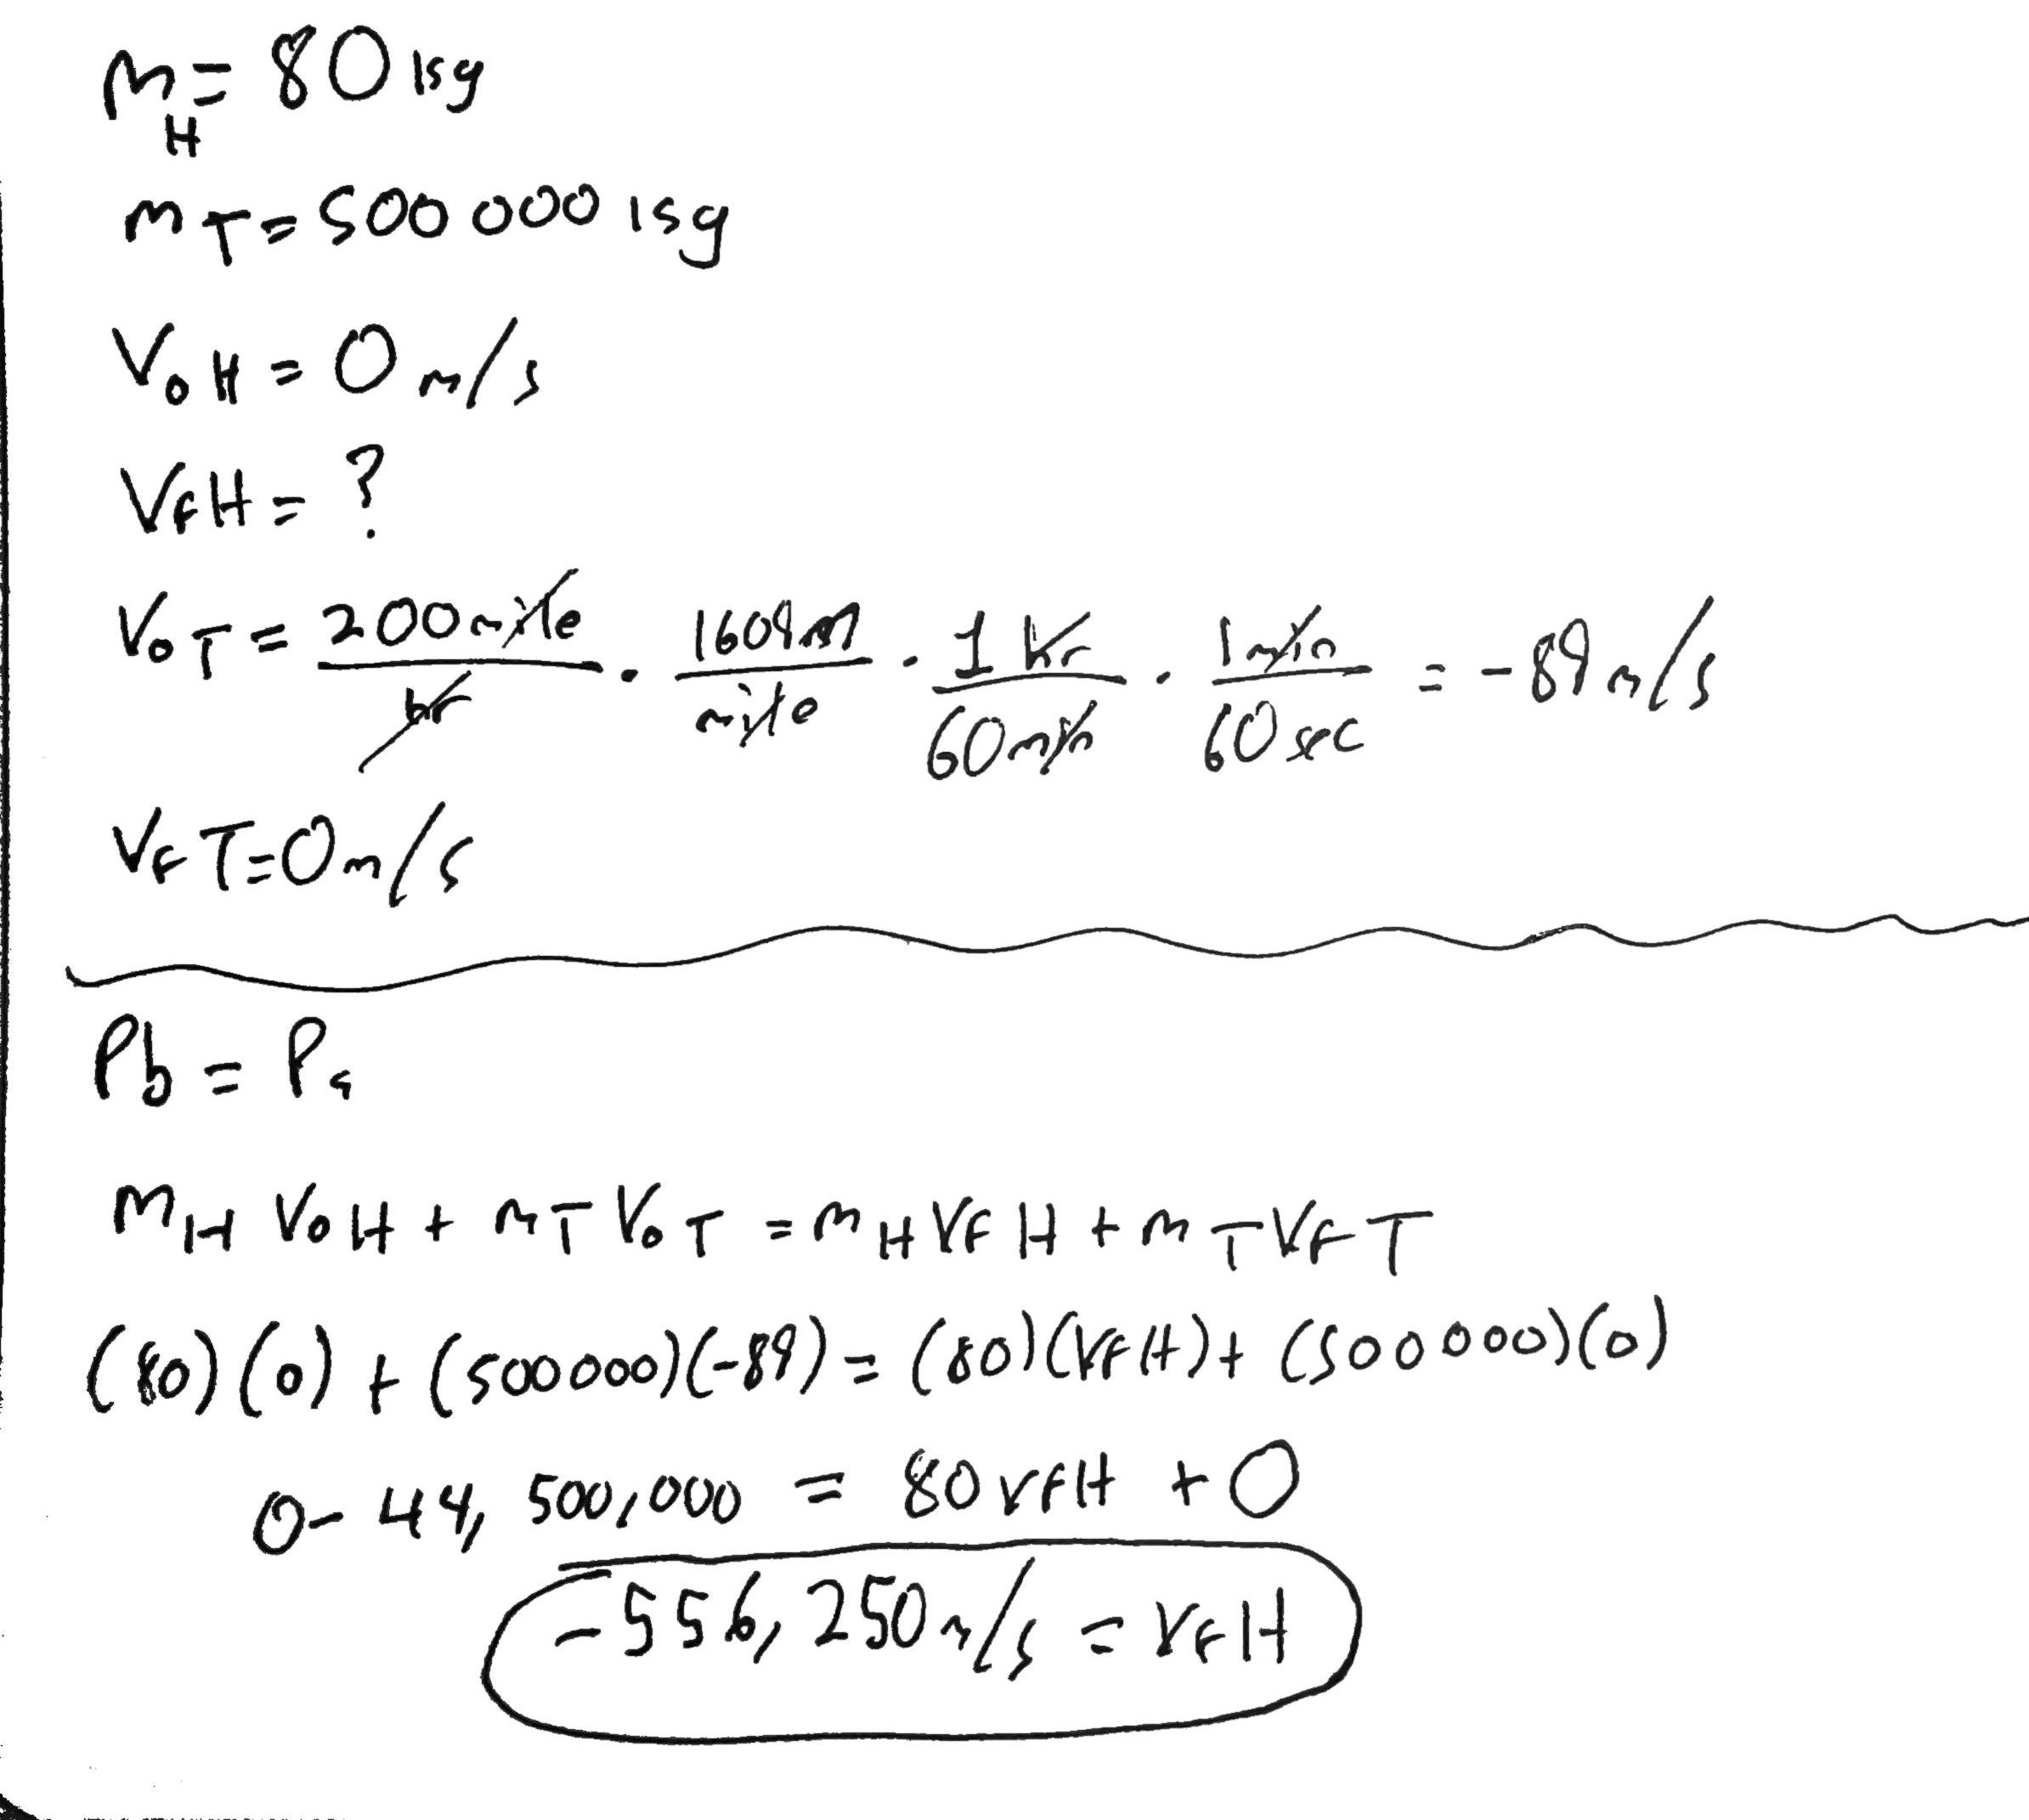
\includegraphics[width=0.6\textwidth]{U4_P1_A.jpg} % Example of adding a figure
\end{figure} 

\newpage

\noindent\textbf{B) Rank the following scenarios as to which will produce the greatest force by Hancock on the train from least to greatest. Explain your reasoning } \\

Scenario A: The train is moving at 60 m/s and the collision lasts 2 seconds.

Scenario B: The train is moving at 50 m/s and the collision lasts 3 seconds.

Scenario C: The train is moving at 100 m/s and the collision lasts 1 second.

Scenario D: The train is moving at 40 m/s and the collision lasts 5 seconds.




\begin{figure}[H]
    \centering
    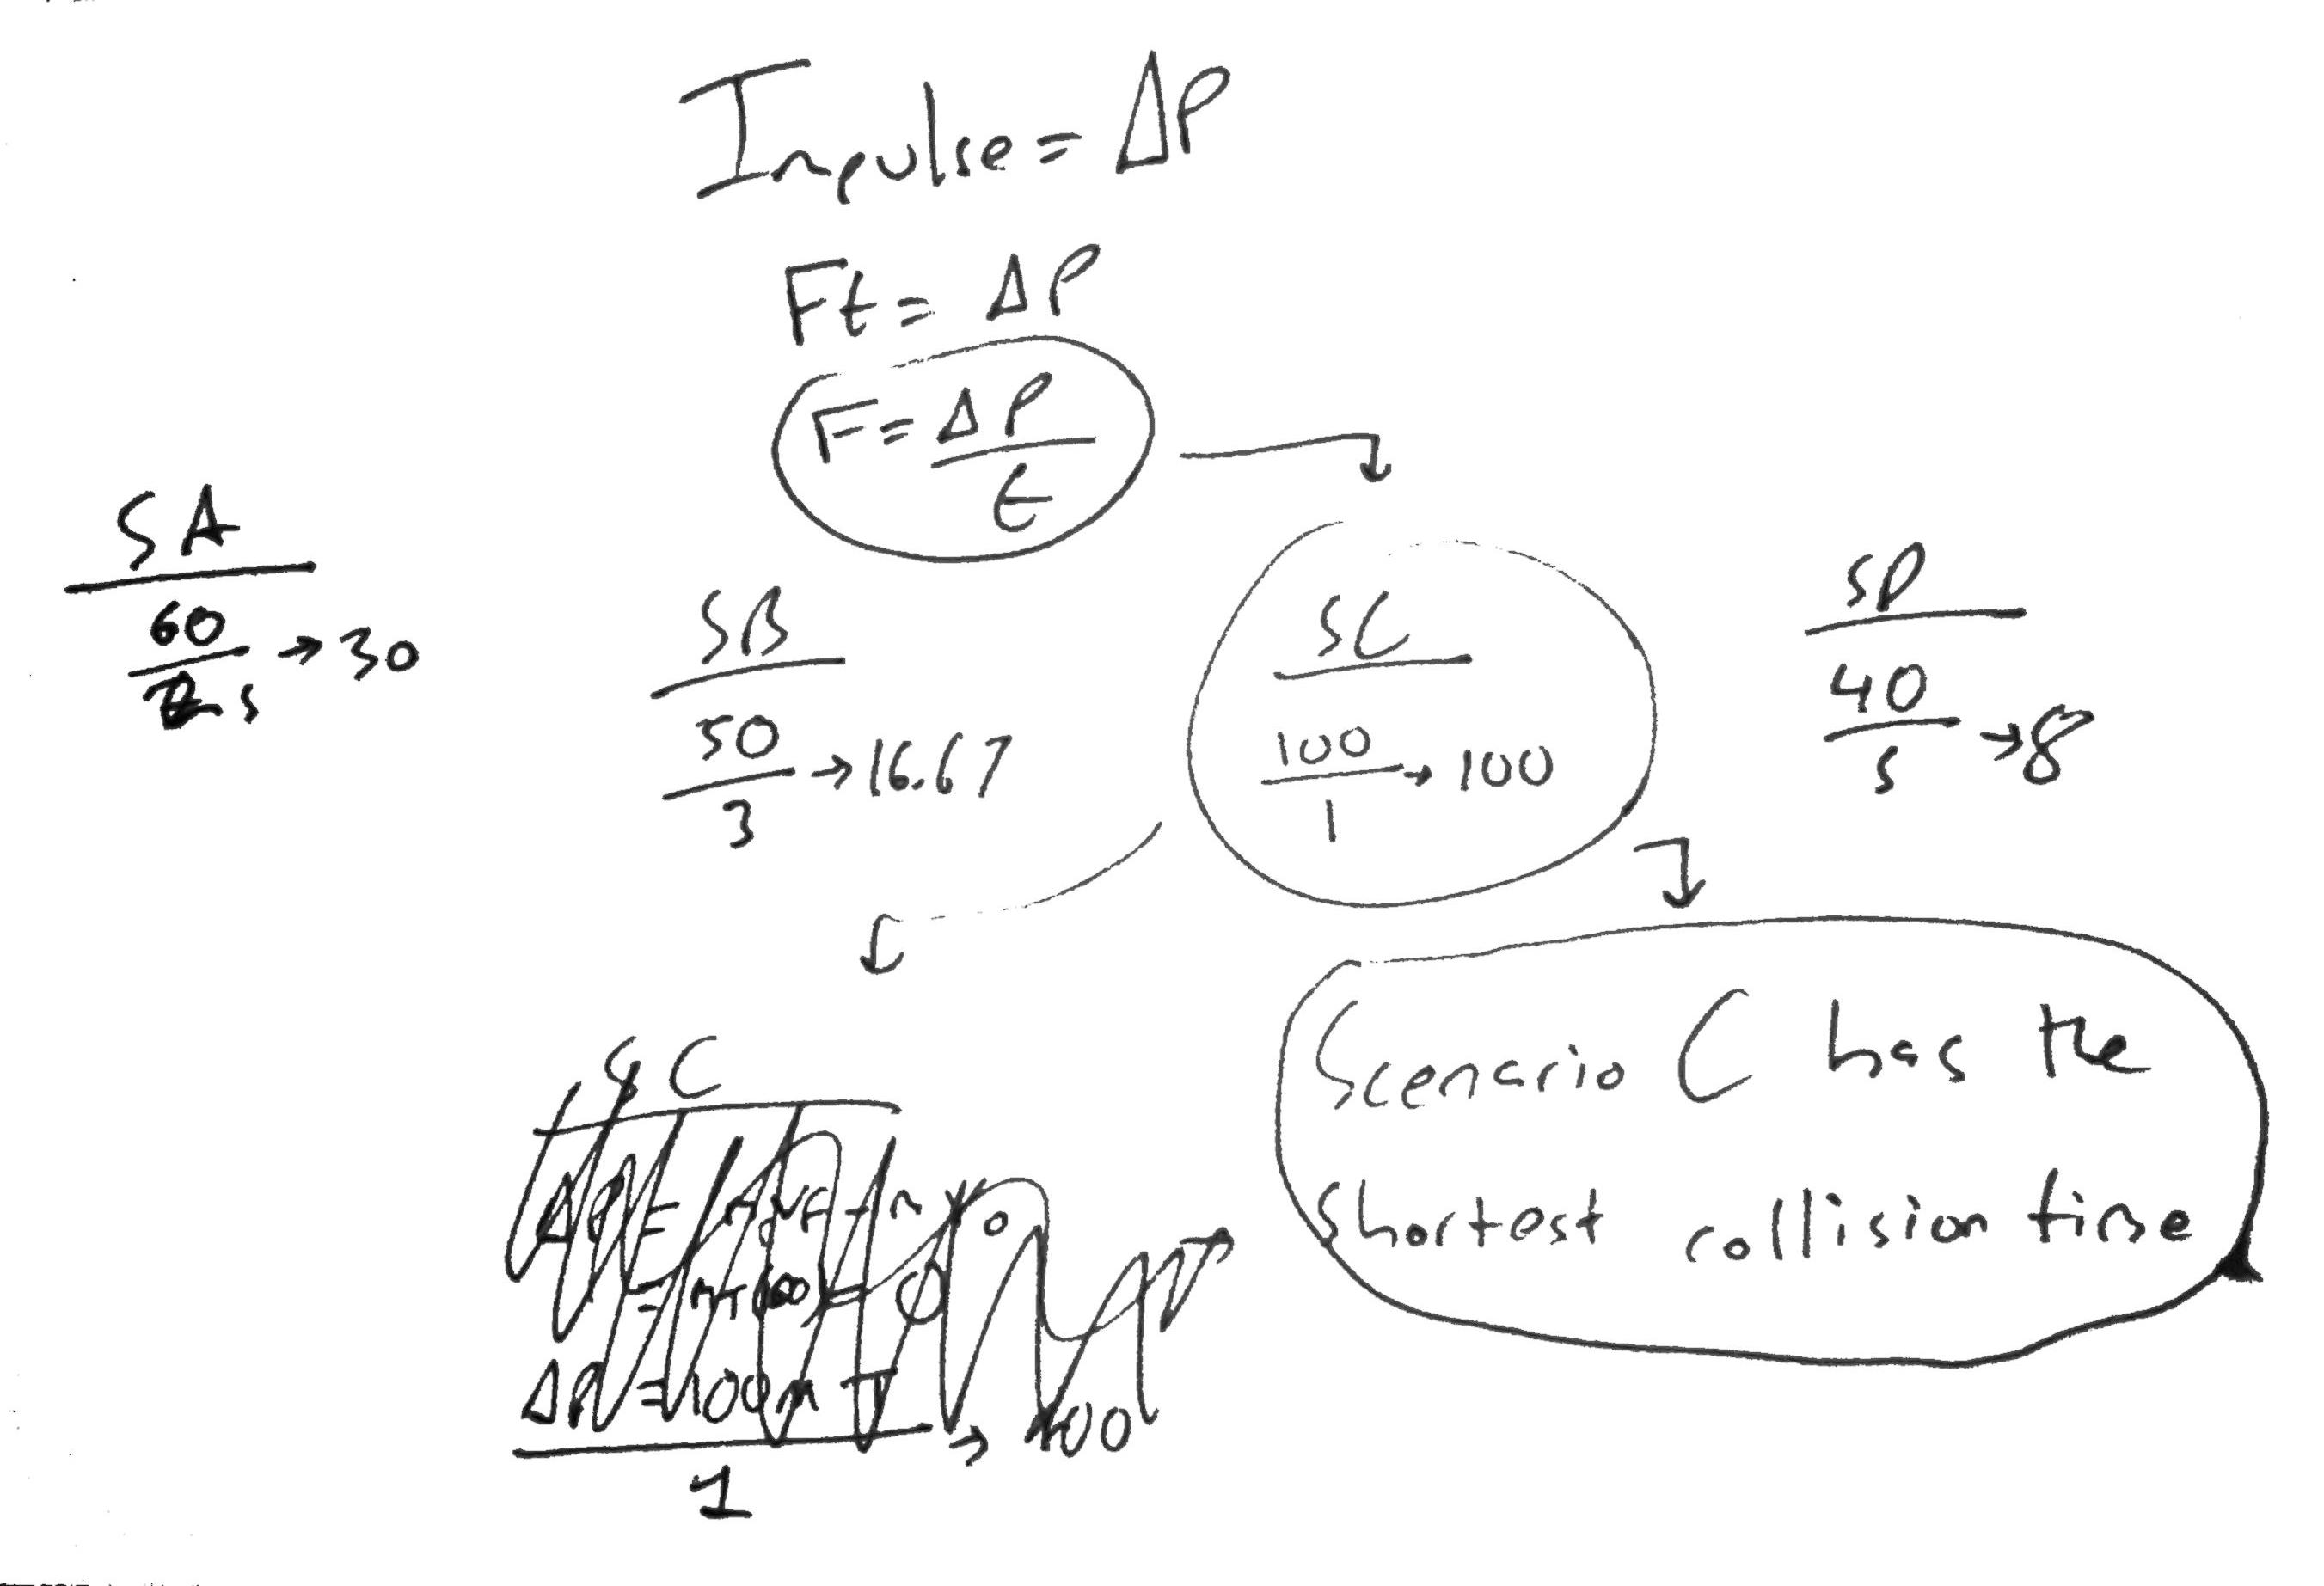
\includegraphics[width=0.7\textwidth]{U4_P1_B.jpg} % Example of adding a figure
\end{figure} 


\noindent\textbf{C) Below is a list of four possible sets of initial and final momenta and kinetic energies of Hancock and the train. Which is the only set that could occur? } \\


\begin{figure}[H]
    \centering
    \includegraphics[width=0.5\textwidth]{} % Example of adding a figure
\end{figure} 


\newpage

\subsection{Problem 2}

The force of Hancock's impact causes the wheels on the track to experience a rotational motion as they are brought to rest. The wheels have a radius of 20 inches and have a constant angular velocity before the collision.

\noindent\textbf{A) Assume the wheels of the train spun with a speed of 75 rev/min before the collision. If Hancock's collision brings the wheels to rest in 2 seconds: 1), what is the angular acceleration, 2) what is the tangential acceleration?} \\


\begin{figure}[H]
    \centering
    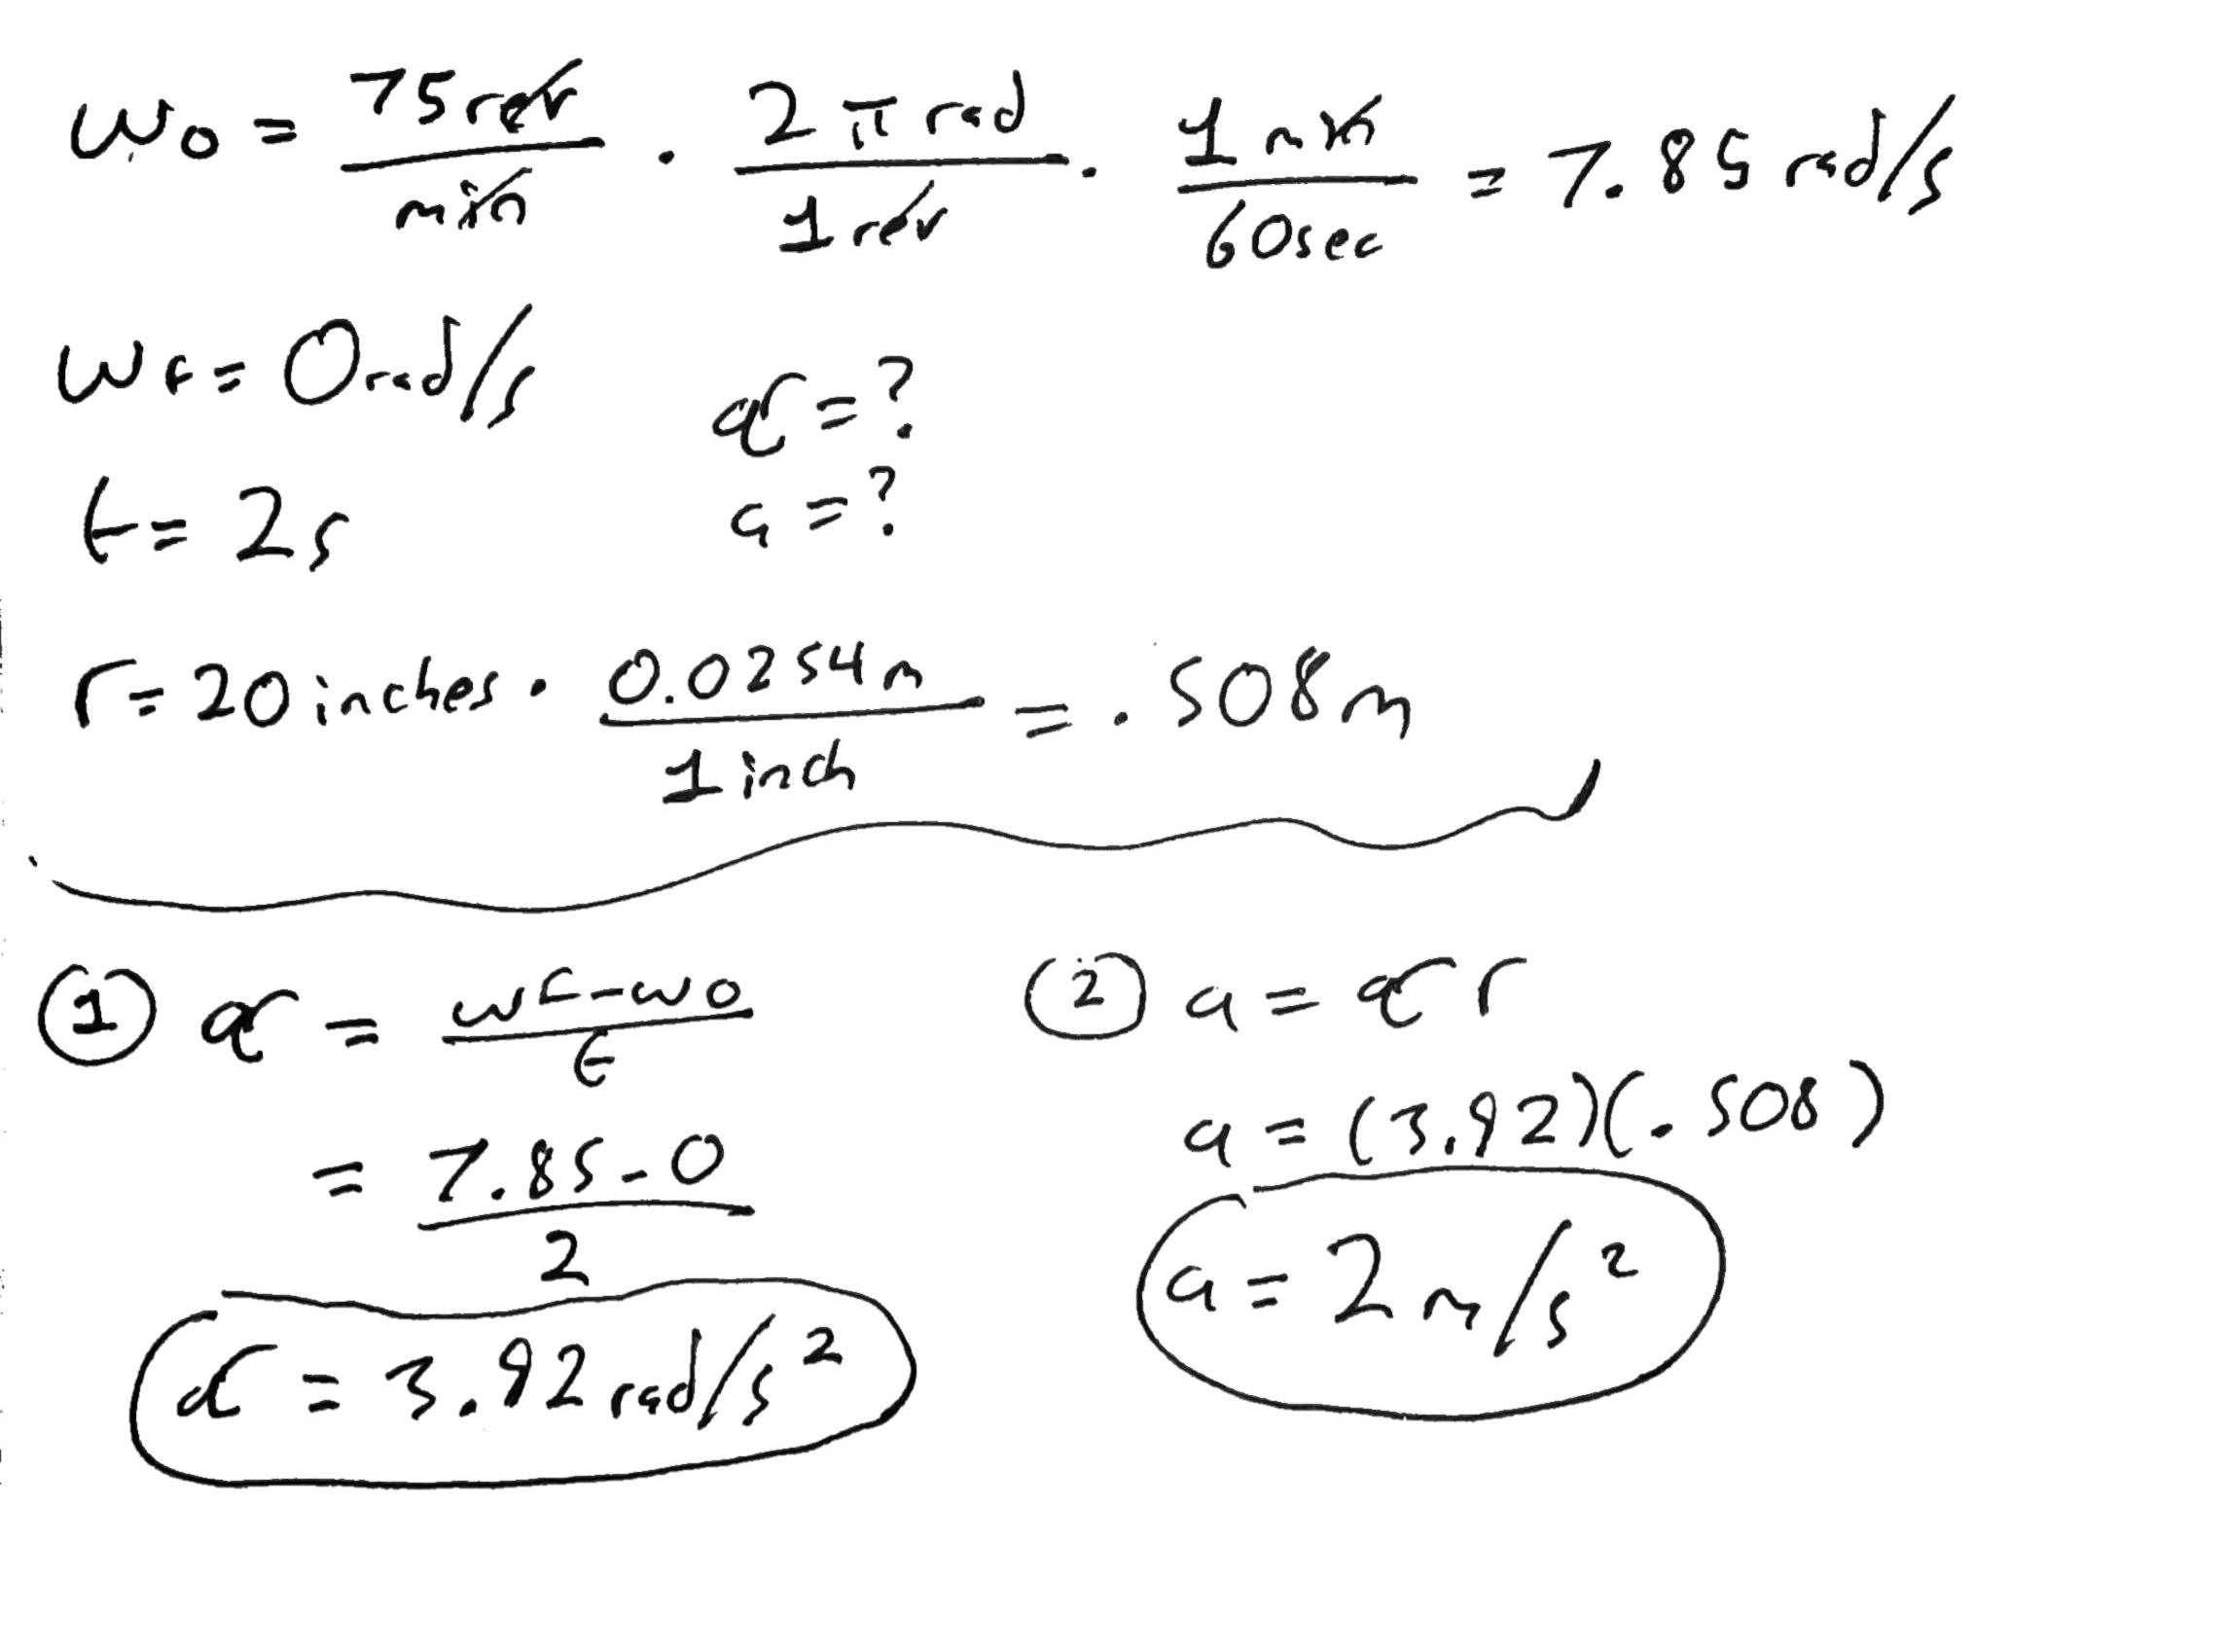
\includegraphics[width=0.6\textwidth]{U4_P2_A.jpg} % Example of adding a figure
\end{figure} 


\noindent\textbf{B) Which of the following angular acceleration vs time graphs best represents the wheels?} \\


\begin{figure}[H]
    \centering
    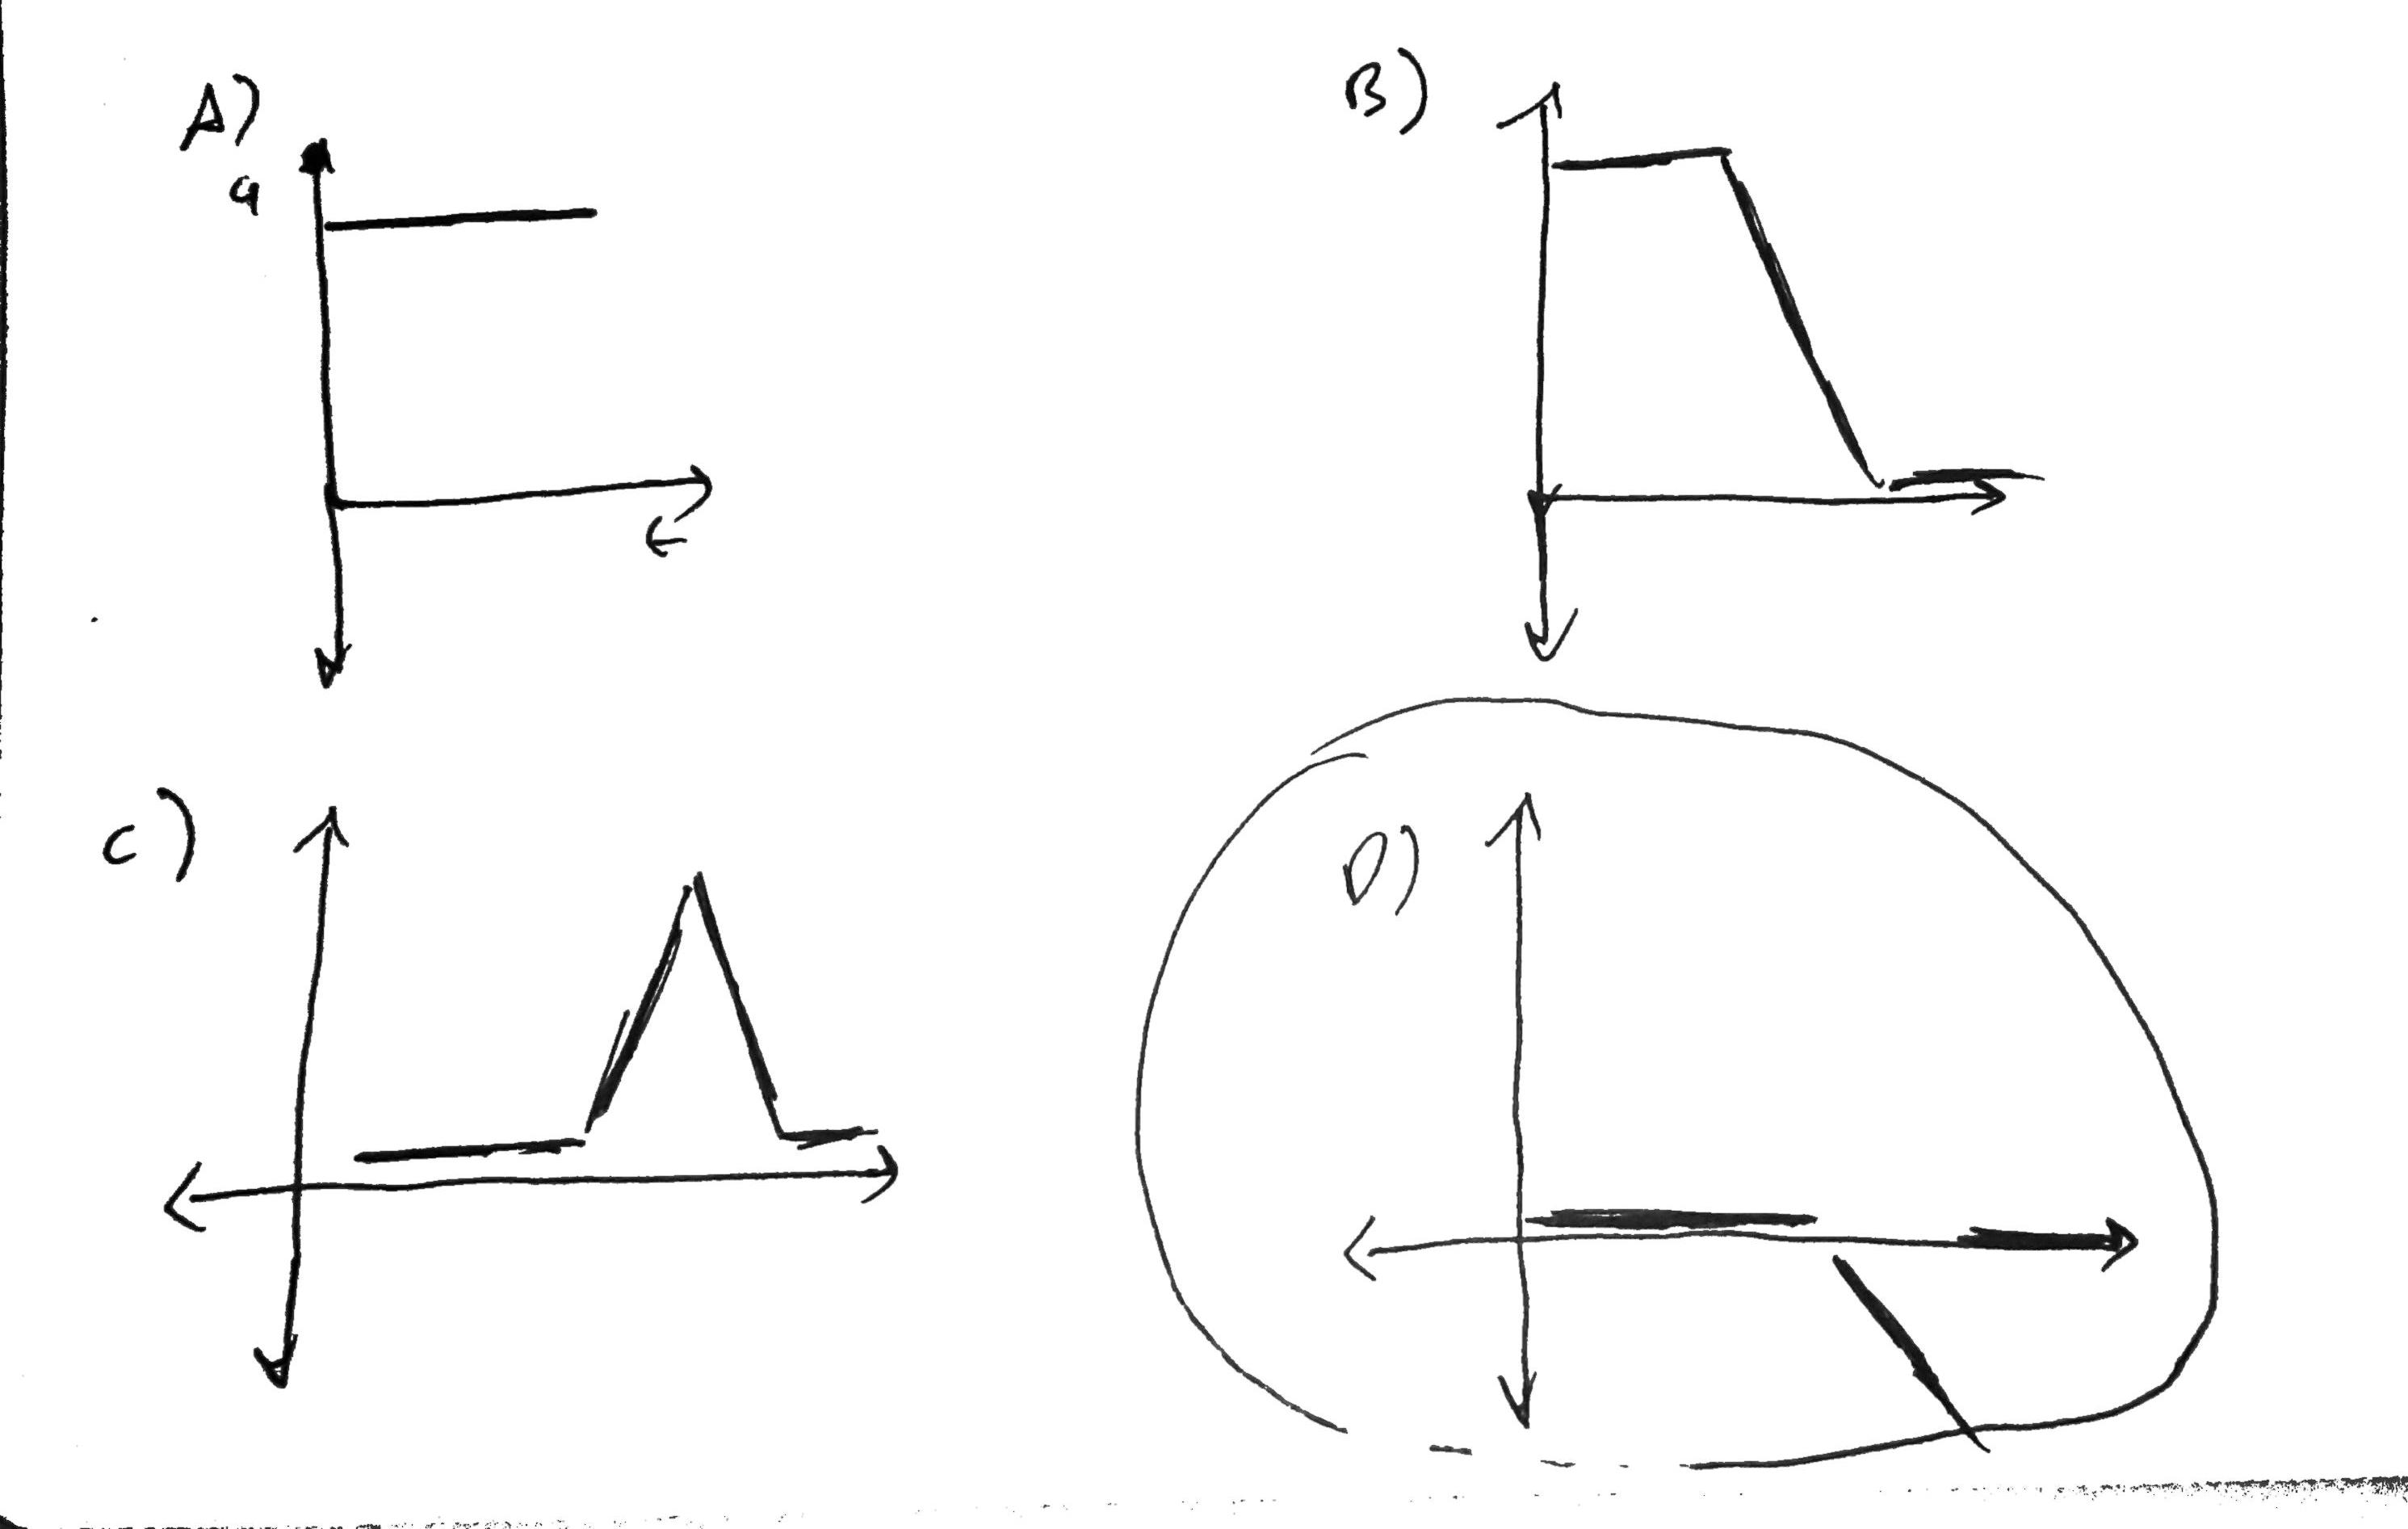
\includegraphics[width=0.6\textwidth]{U4_P2_B.jpg} % Example of adding a figure
\end{figure} 


\newpage
%=====================UNIT 5===================%

\section{Unit 5}

\vspace{-0.5cm}
\singlespacing

\subsection{Scene Analysis}

\textbf{Duration}: 5:00 - 5:52

\vspace{0.3cm}
\noindent\textbf{Summary:} \par
After pursuing criminals in a runwaway vehicle, Hancock decides to put the fear of God into them and throws the car around like a toy in the air, dropping it and catching it a few times. At the end, he uses his legs to push the car onto a spike on a large building. 
\par


\vspace{0.3cm}
\noindent\textbf{Concepts Demonstrated} \par
Hancock grabbing the car by the very end to flip and throw it around like he does could be a demonstration of torque. He's grabbing the car at a point quite away from its center of mass allowing him to rotate more easily. The spike also causes a torque on the car after because of how Hancock pushes it in. The distribution of mass in the car, with the criminals being grouped towards the front, could also be used as an opportunity to discuss moment of inertia. 

\subsection{Problem 1}
Assume the combined weight of the criminals in the car is 240 lbs, and Hancock impales the spike through the center of the car instead of the hood.

\noindent\textbf{A) If the criminals move 0.3 meters from the center of the car towards the front, what is the torque applied to the car? } \\


\begin{figure}[H]
    \centering
    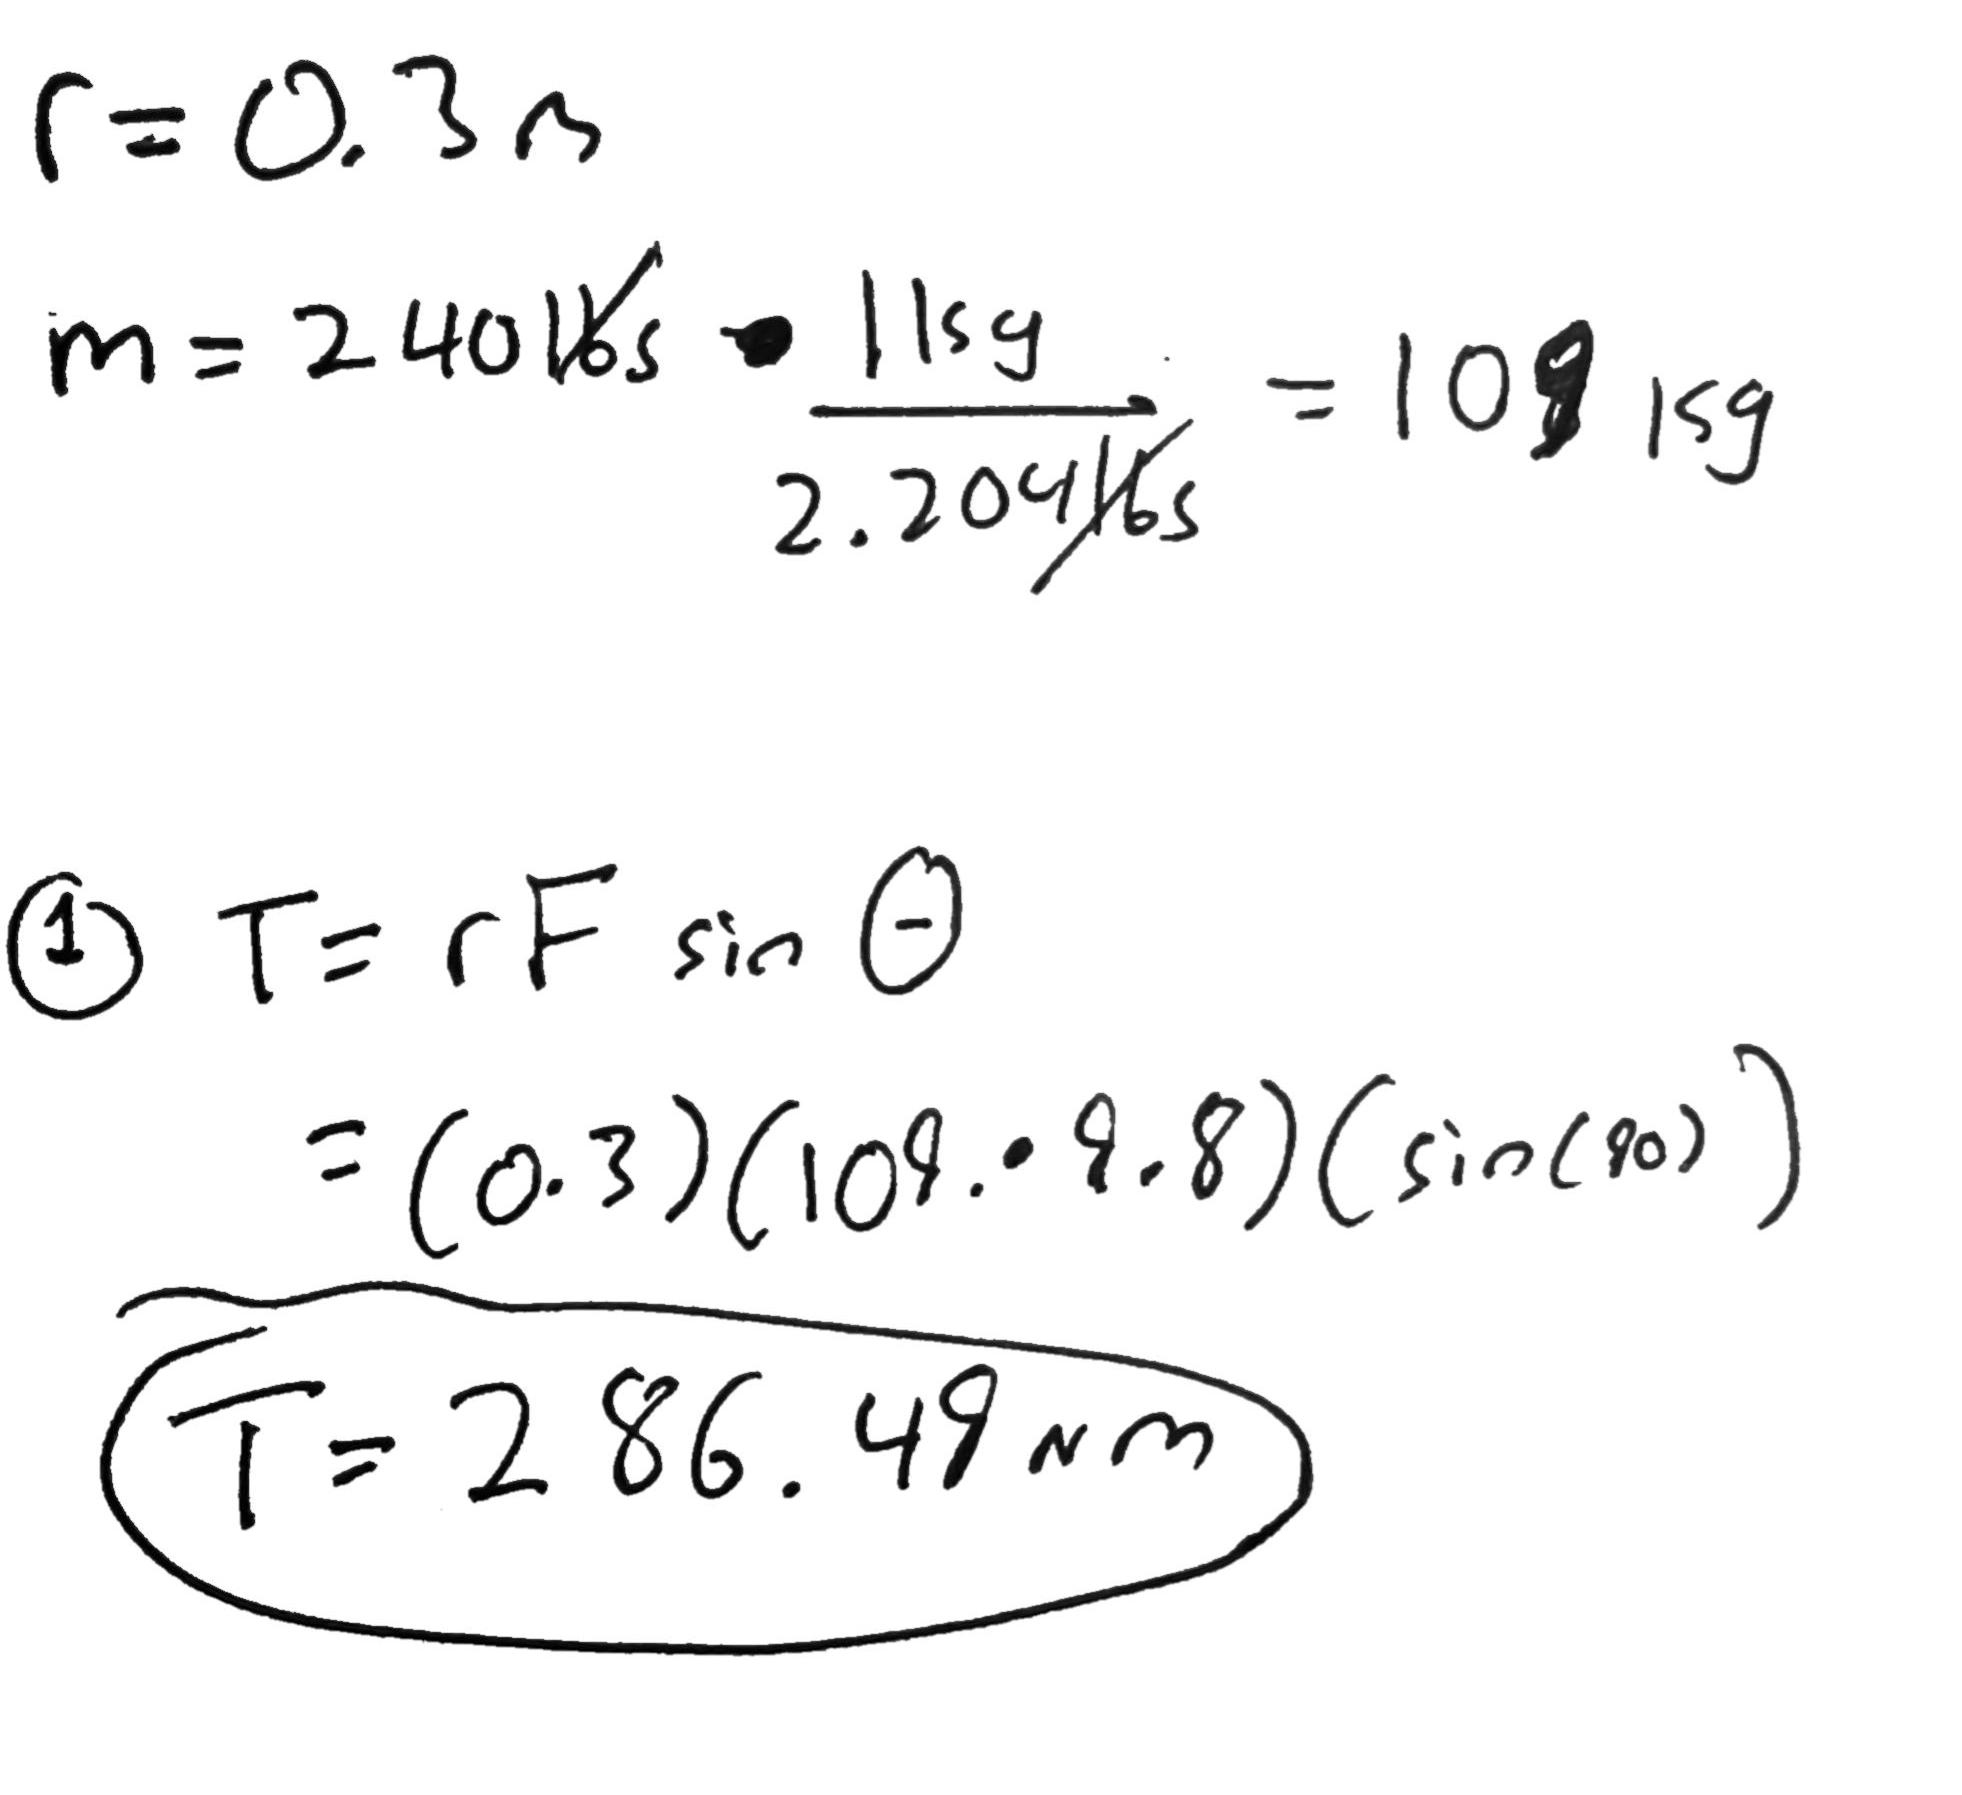
\includegraphics[width=0.6\textwidth]{U5_P1_A.jpg} % Example of adding a figure
\end{figure} 

\newpage

\noindent\textbf{B) If the moment of inertia is 1000kgm$^2$, what is the angular acceleration of the car?} \\


\begin{figure}[H]
    \centering
    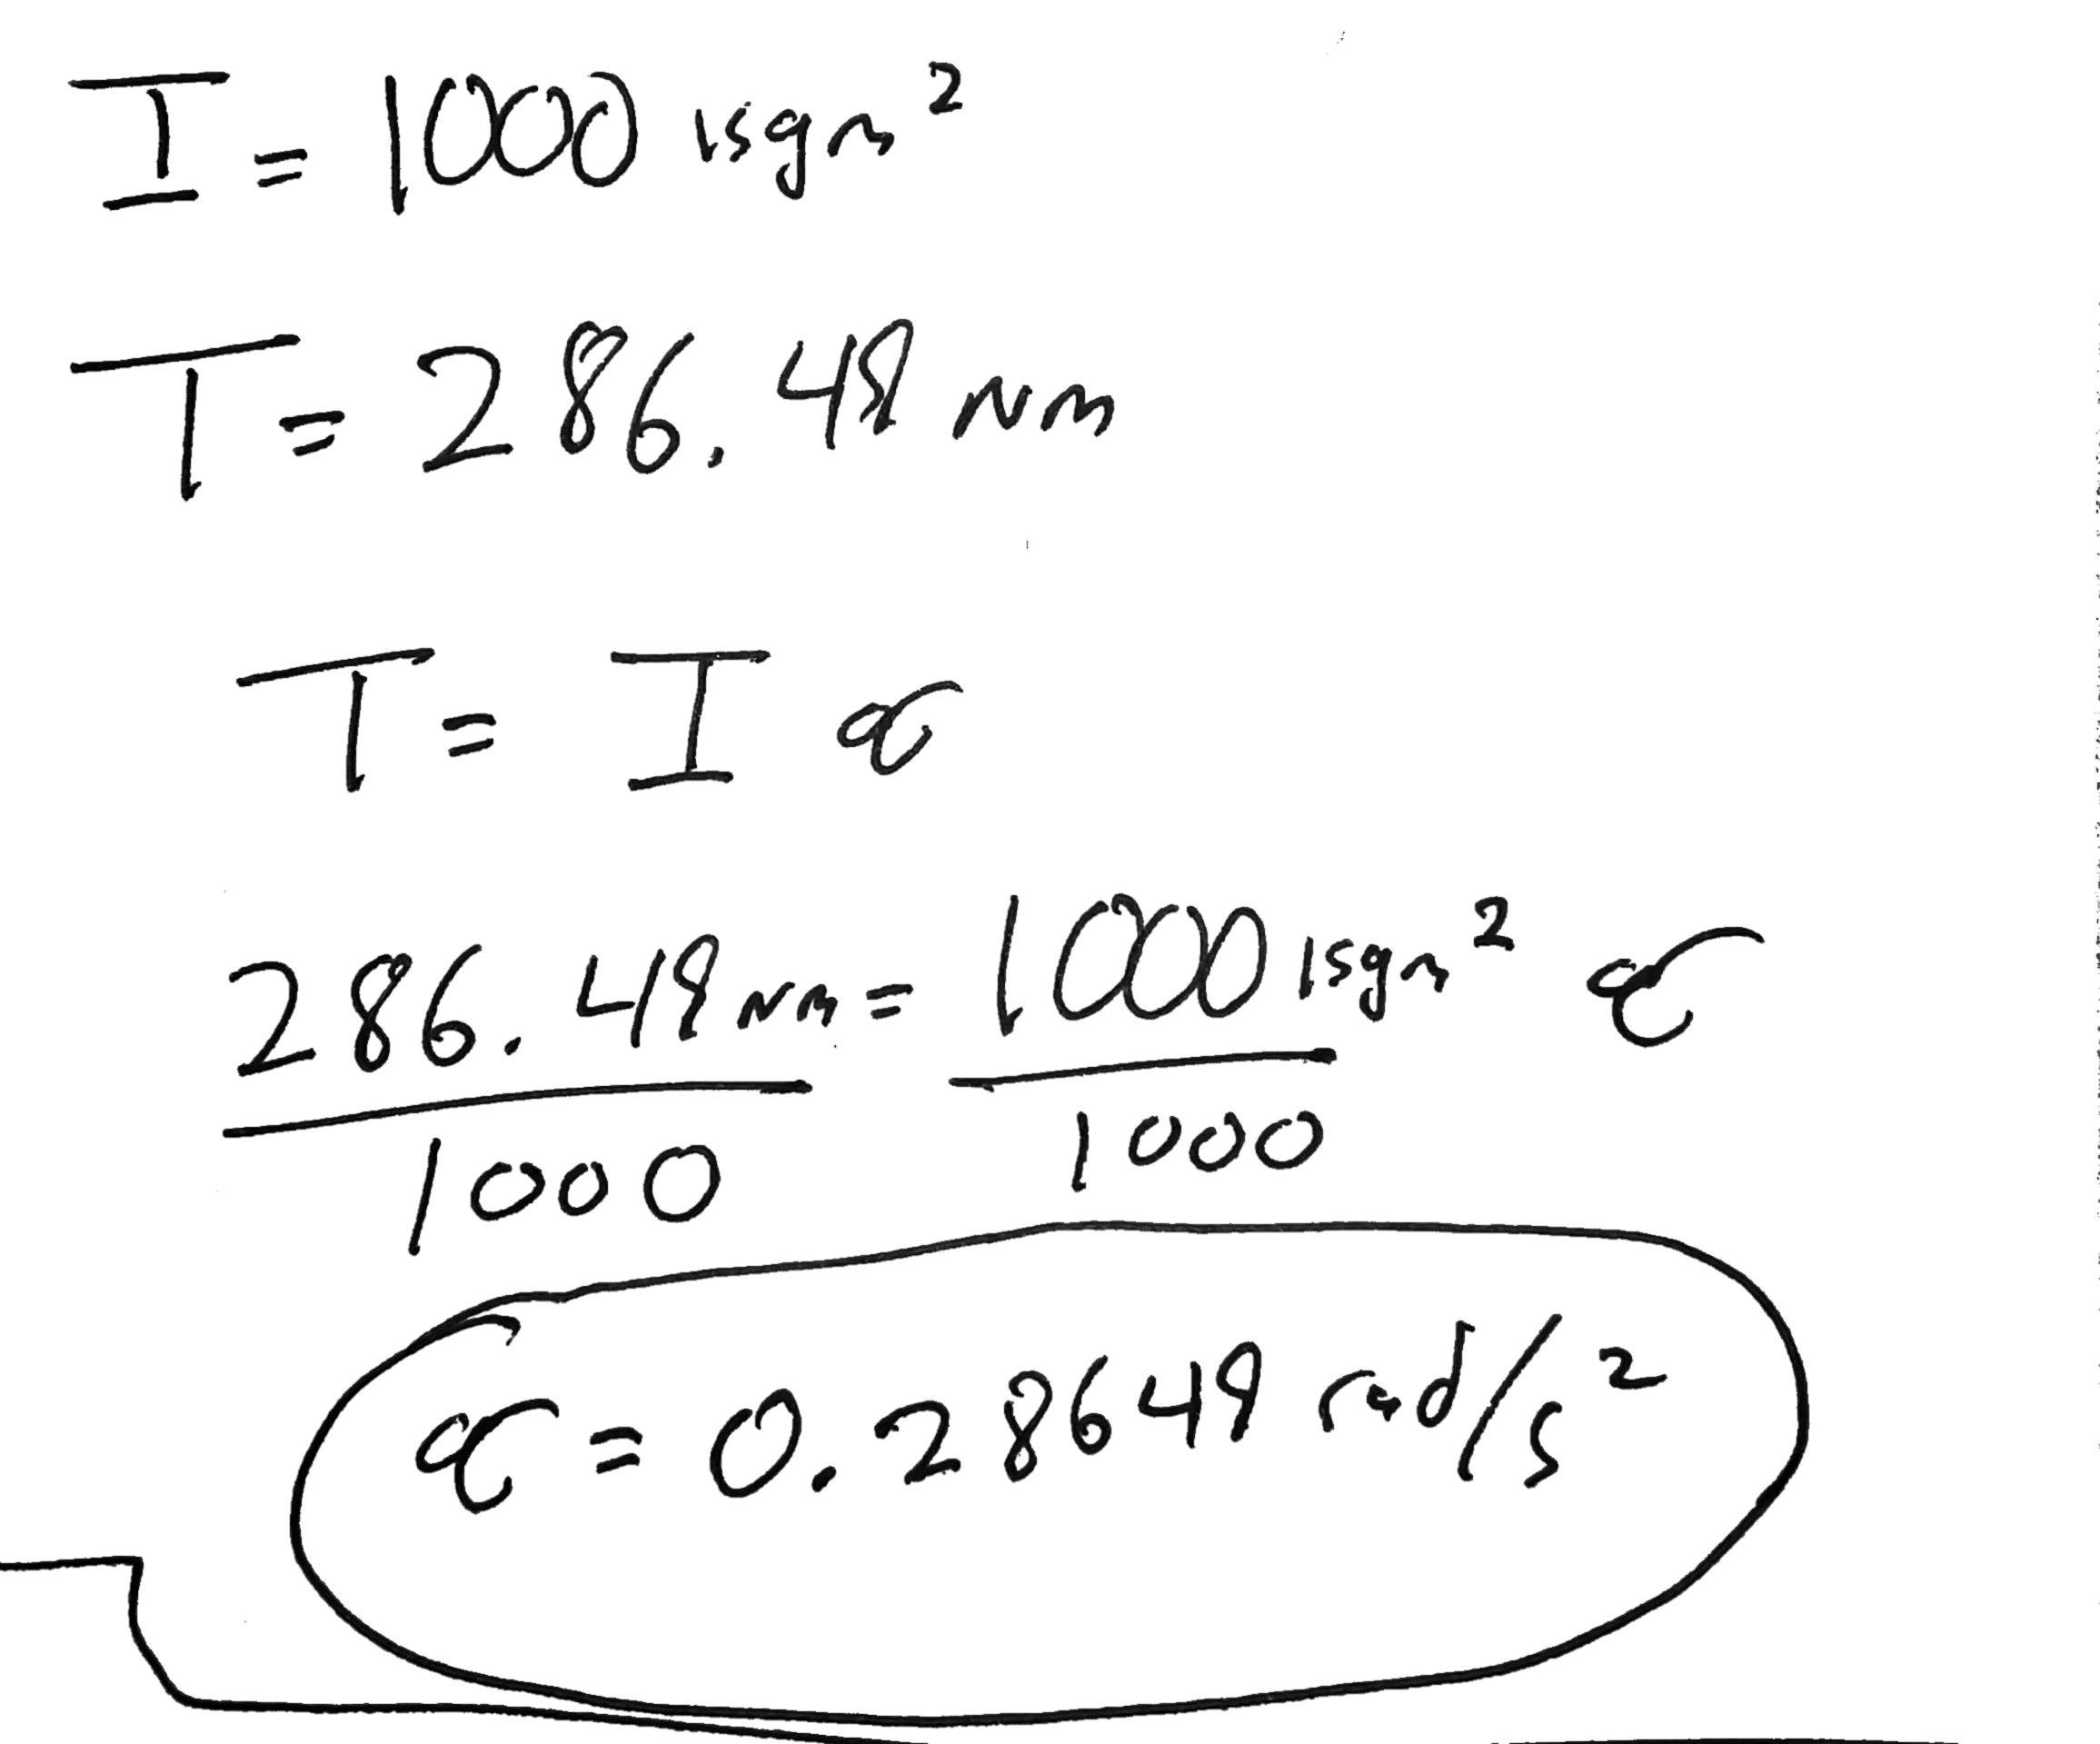
\includegraphics[width=0.8\textwidth]{U5_P1_B.jpg} % Example of adding a figure
\end{figure} 


\noindent\textbf{C) If the criminals remained at the center of the car, how would the torque they apply change if the car was impaled through the hood instead?} \\


\begin{figure}[H]
    \centering
    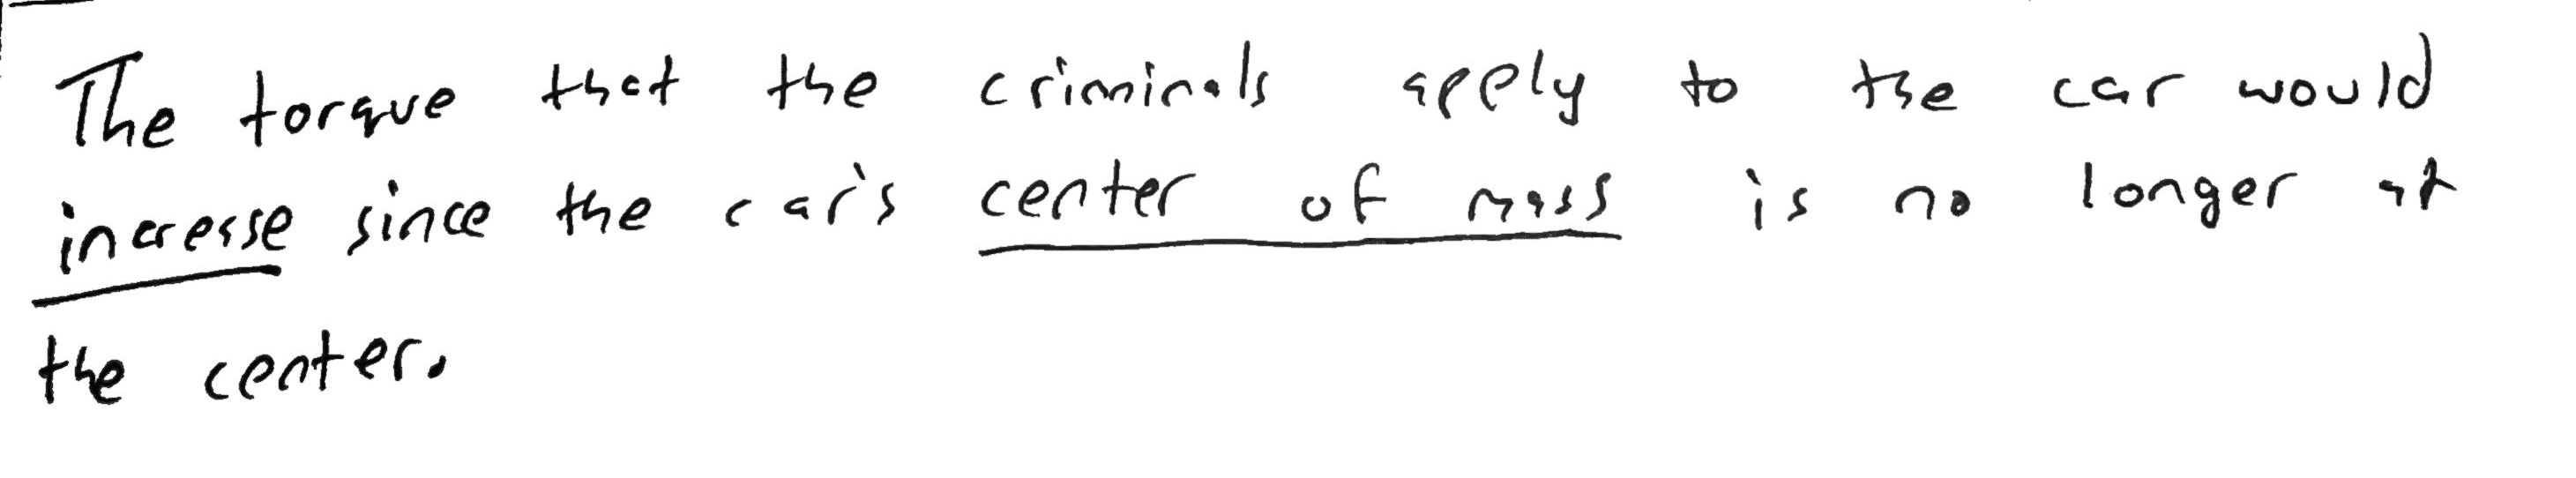
\includegraphics[width=1\textwidth]{U5_P1_C.jpg} % Example of adding a figure
\end{figure} 

\end{document}
